%%% Hlavní soubor. Zde se definují základní parametry a odkazuje se na ostatní části. %%%

%% Verze pro jednostranný tisk:
% Okraje: levý 40mm, pravý 25mm, horní a dolní 25mm
% (ale pozor, LaTeX si sám přidává 1in)
\documentclass[12pt,a4paper]{report}
\setlength\textwidth{145mm}
\setlength\textheight{247mm}
\setlength\oddsidemargin{15mm}
\setlength\evensidemargin{15mm}
\setlength\topmargin{0mm}
\setlength\headsep{0mm}
\setlength\headheight{0mm}
% \openright zařídí, aby následující text začínal na pravé straně knihy
\let\openright=\clearpage

%% Pokud tiskneme oboustranně:
% \documentclass[12pt,a4paper,twoside,openright]{report}
% \setlength\textwidth{145mm}
% \setlength\textheight{247mm}
% \setlength\oddsidemargin{15mm}
% \setlength\evensidemargin{0mm}
% \setlength\topmargin{0mm}
% \setlength\headsep{0mm}
% \setlength\headheight{0mm}
% \let\openright=\cleardoublepage

%% Použité kódování znaků: obvykle latin2, cp1250 nebo utf8:
\usepackage[utf8x, utf8]{inputenc}

%% Ostatní balíčky
\usepackage[english]{babel}
\usepackage{graphicx}
\usepackage{booktabs}
\usepackage{natbib}
\usepackage{mathptmx}
%\usepackage[charter]{mathdesign}
\bibpunct{(}{)}{;}{a}{,}{,}
\usepackage{ucs}
\usepackage{setspace}

\usepackage{amsmath}
\usepackage{amsfonts}
\usepackage{amssymb}
\usepackage{tikz}
\usepackage{booktabs}
\usepackage[nottoc]{tocbibind}

\DeclareMathOperator*{\argmax}{arg\,max}

\usepackage[hyphens]{url}
\usepackage[unicode]{hyperref}   % Musí být za všemi ostatními balíčky
\hypersetup{
    unicode=true,          % non-Latin characters in Acrobat’s bookmarks
    pdftitle={Acquisition of inflectional paradigms with minimal supervision},    % title
    pdfauthor={Radoslav Klíč},     % author
    pdfsubject={Acquisition of inflectional paradigms with minimal supervision},   % subject of the document
    pdfcreator={Radoslav Klíč},   % creator of the document
    pdfkeywords={morphological analysis}, % list of keywords
    pdfstartview={FitH},   %fit horizontally
    colorlinks=true,       % false: boxed links; true: colored links
    linkcolor=black,          % color of internal links
    citecolor=black,        % color of links to bibliography
    filecolor=black,      % color of file links
    urlcolor=blue           % color of external links
}

\newcommand{\todoa}[1]{[\textbf{TODOA} #1]}
\newcommand{\todob}[1]{[\textbf{TODOB} #1]}
\newcommand{\todoc}[1]{[\textbf{TODOC} #1]}

\newcommand{\gloss}[2]{\emph{#1} `#2'}
\newcommand{\supscr}[1]{$^\mathrm{#1}$}
\newcommand{\subscr}[1]{$_\mathrm{#1}$}
\newcommand{\e}[1]{\textit{#1}} % language expressions, examples
\newcommand{\ttt}[1]{\texttt{#1}}
\newcommand{\tbf}[1]{\textbf{#1}}
\newcommand{\eg}{e.g.,~}
\newcommand{\fromTo}[2]{\emph{#1} $\rightarrow$ \emph{#2}}

%%% Drobné úpravy stylu

% Tato makra přesvědčují mírně ošklivým trikem LaTeX, aby hlavičky kapitol
% sázel příčetněji a nevynechával nad nimi spoustu místa. Směle ignorujte.
%\makeatletter
%\def\@makechapterhead#1{
%  {\parindent \z@ \raggedright \normalfont
%   \Huge\bfseries \thechapter. #1
%   \par\nobreak
%   \vskip 20\p@
%}}
%\def\@makeschapterhead#1{
%  {\parindent \z@ \raggedright \normalfont
%   \Huge\bfseries #1
%   \par\nobreak
%   \vskip 20\p@
%}}
%\makeatother

% Toto makro definuje kapitolu, která není očíslovaná, ale je uvedena v obsahu.
\def\chapwithtoc#1{
\chapter*{#1}
\addcontentsline{toc}{chapter}{#1}
}

\begin{document}

% Trochu volnější nastavení dělení slov, než je default.
\lefthyphenmin=2
\righthyphenmin=2

%%% Titulní strana práce

\pagestyle{empty}
\begin{center}

\large

Charles University in Prague

\medskip

Faculty of Mathematics and Physics

\vfill

{\bf\Large MASTER'S THESIS}

\vfill

\centerline{\hspace{18mm}\mbox{
\includegraphics[width=60mm]{logo.pdf}}}

\vfill
\vspace{5mm}

{\LARGE Radoslav Klíč}

\vspace{15mm}

% Název práce přesně podle zadání
{\LARGE\bfseries Acquisition of inflectional paradigms with minimal supervision}

\vfill

% Název katedry nebo ústavu, kde byla práce oficiálně zadána
% (dle Organizační struktury MFF UK)
Institute of Formal and Applied Linguistics

\vfill

\begin{tabular}{rl}

Supervisor of the master's thesis: & RNDr. Jiří Hana Ph.D.\\
\noalign{\vspace{2mm}}
Study programme: & Computer Science\\
\noalign{\vspace{2mm}}
Specialisation: & Computational and Formal Linguistics\\
\end{tabular}

\vfill

% Zde doplňte rok
Prague 2012

\end{center}

\newpage

%%% Následuje vevázaný list -- kopie podepsaného "Zadání diplomové práce".
%%% Toto zadání NENÍ součástí elektronické verze práce, nescanovat.

%%% Na tomto místě mohou být napsána případná poděkování (vedoucímu práce,
%%% konzultantovi, tomu, kdo zapůjčil software, literaturu apod.)

\openright
\onehalfspacing
\noindent
I would like to thank my supervisor, doctor Hana, for professional guidance, a lot of useful advice and setting an example of a professional scientist to me.

\newpage

%%% Strana s čestným prohlášením k diplomové práci

\vglue 0pt plus 1fill

\noindent
I declare that I carried out this master's thesis independently, and only with the cited sources, literature and other professional sources.

\medskip\noindent
I understand that my work relates to the rights and obligations under the Act No. 121/2000 Coll., the Copyright Act, as amended, in particular the fact that the Charles University in Prague has the right to conclude a license agreement on the use of this work as a school work pursuant to Section 60 paragraph 1 of the Copyright Act.

\vspace{10mm}

\hbox{\hbox to 0.5\hsize{%
In ........ date ............
\hss}\hbox to 0.5\hsize{%
signature
\hss}}

\vspace{20mm}
\newpage

%%% Povinná informační strana diplomové práce
\singlespacing
\vbox to 0.5\vsize{
\setlength\parindent{0mm}
\setlength\parskip{5mm}

Název práce:
Automatické osvojení vzorů s minimální supervizí
% přesně dle zadání

Autor: Radoslav Klíč

Katedra: Ústav formální a aplikované lingvistiky (ÚFAL)


Vedoucí diplomové práce:
RNDr. Jiří Hana Ph.D., ÚFAL
% dle Organizační struktury MFF UK, případně plný název pracoviště mimo MFF UK

\onehalfspacing
Abstrakt:
Diplomová práce popisuje algoritmus pro automatické osvojení vzorů s minimální supervizí, který vznikl rozšířením systému Paramor \citep{monson09}, fungujícího zcela bez supervize. Systém je modifikován, aby přijímal snadno dostupná data ve formě ohýbaných slov s označenou hranicí morfémů jako dodatečný vstup. Součástí práce je také knihovna pro hierarchické shlukování, která umožňuje kombinaci různých zdrojů informací. Přístup byl testován na češtině, slovin\-šti\-ně, němčině a katalánštině a vykázal zvýšenou F-míru v porovnáni se základním Paramorem.

Klíčová slova:
strojové učení, morfologie, fonologie, vzory ohýbaní slov
\onehalfspacing
\vss}\nobreak\vbox to 0.49\vsize{
\setlength\parindent{0mm}
\setlength\parskip{5mm}

Title:
Acquisition of inflectional paradigms with minimal supervision

Author:
Radoslav Klíč

Department:
Institute of Formal and Applied Linguistics
% dle Organizační struktury MFF UK v angličtině

Supervisor:
RNDr. Jiří Hana Ph.D., Institute of Formal and Applied Linguistics

\onehalfspacing
Abstract:
The thesis presents a semi-supervised morphology learner developed by extending Paramor \citep{monson09}, an unsupervised system, to accept easy to obtain manually provided data in the form of inflections with marked morpheme boundary. In addition, a hierarchical clustering framework allowing combination of multiple sources of information was developed as a part of the thesis. The approach was tested on Czech, Slovene, German and Catalan and has shown increased F-measure in comparison with the Paramor baseline.

Keywords:
machine learning, morphology, phonology, inflectional paradigms

\vss}

\newpage

%% Strana s automaticky generovaným obsahem diplomové práce. U matematických
%% prací je přípustné, aby seznam tabulek a zkratek, existují-li, byl umístěn
%% na začátku práce, místo na jejím konci.
\onehalfspacing
\openright
\pagestyle{plain}
\setcounter{page}{1}
\tableofcontents

\chapter{Introduction}

Morphological analysis is important for many applications working with natural language in written or spoken form. An analyser can be built manually (for example, using finite-state technology) or machine learning (ML) with various levels of supervision can be employed. Completely supervised techniques and hand-written analysers can achieve very high quality of results. 

However, supervised ML approaches usually require an annotated corpus, which for many of the world's languages is an unavailable resource and it would be expensive or straight out impossible to create one. Similar problem arises with the hand-written analysers, for which experts with deep knowledge of given language and strong linguistic and programming background are needed. Another important resource to be taken into account is time, as creating an analyser manually by experts is considerably time-consuming.

In cases where the expensive resources are not available, one may use one of the unsupervised or semi-supervised morphology learners. The semi-supervised approaches are attempting to use the fact that even for underresourced languages there is (nearly) always possible to get some useful resources without spending much time or money. These resources may include inflections of individual words or inflection classes from a grammar textbook. 
 
Analyses vary not only in the type and amount of learning data they require, but also in the output they provide to the user. Morphological analysis in its standard sense returns all possible lemmas and part-of-speech tags for each word in the text, disregarding the context. For example, \e{handles} should be analysed as a 3\supscr{rd} person singular verb form and a plural noun; using the Penn Treebank tagset \citep{marcus93} this could be encoded as \{(\e{handle}, VBZ), (\e{handle}, NNS)\}. Resource-light approaches to MA are not always able to provide such detailed analysis, but can produce results such as:

 \begin{enumerate}
\item Related word forms. For \emph{run}, the analyser may return \emph{runs}, \emph{running}. This kind of analysis is useful in information retrieval. For example, if you search for \emph{table} on Google, you expect it to find  \emph{tables} as well.
\item Morphemic segmentation, i.e. splitting words into morphemes. For \emph{tables},  \emph{table} + \emph{s} is returned. Speech recognition systems can benefit from this kind of analysis by building morpheme level language models.
\end{enumerate}

The system developed for this thesis is semi-supervised as it uses manually entered inflections with marked morpheme boundary as one of its inputs. It contains two almost independent modules: 
\begin{enumerate}
\item \label{li:mod_par} Modified Paramor \citep{monson09} analyser. Modifications aim at improving its results by using the manual seed mentioned above. The seed is used (1) to help Paramor recognise true suffixes and paradigms and (2) generate simple rules capturing stem allomorphy. Treating allomorfic variants as a single stem enables the algorithm to find more complete paradigms and place morpheme boundaries more adequately. Like the original Paramor, the system is capable of inducing inflectional paradigms as well as using them for morphemic segmentation.
\item Word clustering framework which allows combination of multiple sources of information, for example output of a paradigm producing algorithm such as the one from (\ref{li:mod_par}), morphology segmentation algorithm or modified edit distance. It also provides evaluation of resulting clusters' adequacy if a lemmatised corpus is available.
\end{enumerate} 

The target languages are inflectional, especially Slavic languages, but the system should yield acceptable results for any language with suffixal morphology.

\section{Terminology}
Terms from the field of morphology are used quite loosely in various publications. In this section, I briefly summarise some of them and clarify in what sense they will be used in this thesis.

\textbf{Morpheme} is the smallest unit in a language bearing a meaning. It is an abstract entity, which may be realised in speech or writing by more than one form. The individual realisations are called \textbf{morphs}. Every word consist of one or more morphs \eg \e{talk + ing, un + avail + able}.

\textbf{Allomorphs} are morphs realising the same morpheme, depending on the context. They occur due to phonological/graphemic changes or irregularities. For example, consider the declension of the Czech word \e{matka} `mother' in Table \ref{table:matka}. It exhibits stem-final conso\-nant chan\-ge (palatalisation of \e{k} to \e{c}) triggered by the dative and local singular ending, and epenthesis (insertion of \e{-e-}) in the bare stem genitive plural. As a result, the stem has 3 allomorphs: \e{matk}, \e{matc} and \e{matek}.
\begin{table}[htb]
\begin{center}
\begin{tabular}{lll}
\toprule \bf Case & \bf Singular & \bf Plural \\ \midrule
nom & mat\textbf{k}+a & mat\textbf{k}+y \\
gen & mat\textbf{k}+y & mat\textbf{ek}+0 \\
dat & mat\textbf{c}+e & mat\textbf{k}+ám\\
acc & mat\textbf{k}+u & mat\textbf{k}+y \\
voc & mat\textbf{k}+o & mat\textbf{k}+y \\
loc & mat\textbf{c}+e & mat\textbf{k}+ách \\
inst & mat\textbf{k}+ou & mat\textbf{k}+ami \\
\bottomrule
\end{tabular}
\end{center}
\caption{\label{table:matka} Declension of the word \gloss{matka}{mother}. Changing part of the stem is in bold.}
\end{table}

\noindent \textbf{Inflection} is a morphological process which creates different forms of one word:
\begin{quote}
\e{walk, walks, walked, walking}
\end{quote} \tbf{Derivation} is a process which creates new words: \begin{quote}
\e{relent $\rightarrow$ relentless $\rightarrow$ relentlessness}
\end{quote} 

\noindent \textbf{Lexeme} is a set of words related by inflection. For example, all forms of the word \gloss{matka}{mother} in Table \ref{table:matka} form a lexeme. Lexeme is also sometimes used in a related but slightly different meaning -- as a unit of language that has a semantic meaning.

\textbf{Canonical form}, or dictionary form, is a form selected by a convention to represent a lexeme. For example, usually infinitive is chosen for verbs and nominative singular for nouns.

\textbf{Lemma} is a unique identifier for a lexeme. Typically, the canonical form can serve as a lemma (possibly with indexes disambiguating polysemous words, such as \e{bank\subscr{1}}/\e{bank\subscr{2}}). Nevertheless, lemma can be any arbitrarily chosen unique identifier (at least in NLP).

Inflections of most of the words follow regular patterns, called \textbf{paradigms}. Definitions of a paradigm in various works differ. Paradigms as taught in Czech schools consist of suffix for each combination of relevant grammatical categories\footnote{case and number for nouns, person and number for verbs} and a word inflected according to the paradigm. This word serves as an example and an easy-to-remember identifier of the paradigm. In this thesis, the term paradigm will be used for a set of suffixes. 
%For a set of inflections of the same lemma, I will use the term \textbf{l-paradigm}.

\section{Layout of the thesis}
The rest of the thesis is organised as follows: Chapter \ref{chapter:prev_works} reviews some of the important previous works related to the subject of the thesis. Detailed description of Paramor is provided in Chapter \ref{chapter:paramor}. Chapter \ref{chapter:modifications} presents modifications of Paramor to handle basic allomorphy and use a manually provided seed. The clustering framework and implemented string distance measures are described in Chapter \ref{chapter:clustering}. Experiments and their results are presented in Chapter \ref{chapter:results}. Chapter \ref{chapter:conclusion} summarises the thesis and outlines possible future improvements. 

\chapter{Previous Works}\label{chapter:prev_works}
\newcommand{\cprob}[2]{P(#1 | #2)}
The area of computational morphology is wide and rich with publications. Approaches to computational morphology can be roughly classified into 3 basic categories:
\begin{enumerate}
\item Unsupervised morphology learners: algorithms which use solely plain-text corpora or word-lists as their input.

\item Supervised systems and hand-built systems. They require annotated corpora or manually created rules together with large vocabularies.

\item Semi-supervised and resource-light approaches. The individual approaches vary in the amount and form of human supervision. The forms of human supervision may include providing data such as inflected word forms, paradigms, affix lists, phonological rules etc. Human supervisor may also be employed in an iterative training process by being asked to interact in each iteration of the learning process.
\end{enumerate}

In this chapter, some of the existing systems are described, with main focus on the unsupervised and semi-supervised methods.

\section{Creating analysers by experts}
The two most commonly used approaches to creating hand-made morphology analysers are 2-level morphology \citep{Koskenniemi83, Karttunen03} and the so-called ``engineering approach''.

\subsection{Two-level morphology (2LM)}
2LM is a popular formalism, which works with two levels of representation of words: an abstract \emph{lexical level} and a concrete \emph{surface level}, for example:
\begin{quote}\begin{flushleft}
\tt 
b a b y + 0 s\\
b a b i 0 e s
\end{flushleft}
\end{quote} with an inline notation 
\begin{quote}\begin{flushleft}
\tt 
b:b a:a b:b y:i +:0 0:e s:s
\end{flushleft}
\end{quote}
relates the lexical (upper) and surface (lower) form of the word \e{babies} . The + character denotes the morpheme boundary, 0 is an empty string (there has to be a 1:1 correspondence between characters on each level). The two levels are related by declarative context-sensitive rules such as: 
\begin{quote}\begin{flushleft}
\tt 
y:i <= \_ +:0 s:s\\
0:e <= y:i +:0 \_ s:s
\end{flushleft}
\end{quote}
The rules above describe changing of \e{y} to \e{i} before the morpheme boundary followed by \e{s} and insertion of \e{e} between \e{i} and \e{s} (in the specified context). The underscore sign denotes the position where the change is taking place.

The designer of the analyser specifies the rules and a network of lexicons containing morphemes in their lexical form. The network also specifies basic morphotactics of morphemes in the lexicons. Rules and lexicons are then compiled into a finite-state transducer. The formalism is powerful enough to express  most of the phonological and morphological processes, although their description by the rules is not always straightforward.

\subsection{Engineering approach}\label{sec:engineer}
The engineering approach, represented by \citep{hajic-2004-hab}, models morphology as a purely concatenative process. Changing parts of the stem are moved to the suffixes and as a result, high number of paradigms emerge. For example, to model the English past tense one would need to create paradims as (\e{0, ed}), (\e{0, ped}), (\e{0, ted}), (\e{y, ied}) etc.
 Table \ref{table:matka_eng} shows how would an ``engineering'' paradigm for the word \gloss{matka}{mother} look like. (For comparison with the ``linguistic'' paradigm, see Table \ref{table:matka}). 
 
 Positive attributes of the approach are easy implementation, high speed and a well readable morphology specification.

\begin{table}[htb]
\begin{center}
\begin{tabular}{lll}
\toprule \bf Case & \bf Singular & \bf Plural \\ \midrule
nom & mat + ka &  mat + ky \\
gen & mat + ky &  mat + ek \\
dat & mat + ce &  mat + kám\\
acc & mat + ku &  mat + ky \\
voc & mat + ko &  mat + ky \\
loc & mat + ce &  mat + kách \\
inst & mat + kou & mat + kami \\
\bottomrule
\end{tabular}
\end{center}
\caption{\label{table:matka_eng} Engineering approach paradigm for \gloss{matka}{mother}.}
\end{table}

\section{Unsupervised algorithms}
This section presents two representatives of the unsupervised approaches: Goldsmith's Linguistica \citep{goldsmith01}, which returns partial paradigms called \emph{signatures} and Morfessor \citep{creutz-lagus-2002, creutz-lagus-2005, creutz07}, which induces morphemic segmentation of plain-text corpora. Paramor \citep{monson09}, the unsupervised algorithm I have extended in this thesis, is described separately in Chapter \ref{chapter:paramor}.

\subsection{Linguistica}
\cite{goldsmith01} presents Linguistica, an unsupervised approach based on minimum description length (MDL). Basic idea of the approach is to find a morphology model which is compact and allows compact representation of the corpus. More precisely, a model that minimises the sum of the compressed size of the corpus and the compressed size of the model. Assumption is that the model will be close to reality due to the economy of languages. 

Morphology model consists of a stem list, suffix lists and a set of \emph{signatures}. A signature contains stems and suffixes (more precisely, pointers to the respective lists). Their presence together means that all combinations of stems and suffixes in the signature are possible in the given language. A stem can be present only in one signature, occurrence of a suffix in more signatures is possible. A sample of several signatures (without stems) can be found in Table \ref{table:goldsmith-signatures}.

To be able to analyse a word as a stem and more than one suffix, Goldsmith introduces \emph{complex stems}, which consist of three pointers: to a signature, a stem and a suffix. For example, the word \emph{workings} would be analysed as a complex stem \emph{working} (pointers to: stem \emph{work}, suffix \emph{ing}, signature for \emph{working}) + suffix \emph{s}. The algorithm works roughly as follows:
\begin{enumerate}
\item Words are divided into stems and suffixes using probability based heuristics. Signatures are created according to these splits. One of the heuristics is the following: Consider all the tails up to the length 6 and score them by the measure:
\[\frac{C(n_1n_2 \dots n_k)}{N_k} ~ \log \frac{C(n_1n_2 \dots n_k)}{C(n_1) C(n_2) \dots C(n_k)}\]
where $n_1,n_2 \dots n_k$ are individual characters of the tail, $N_k$ denotes the number of all tails of length $k$ and $C(x)$ denotes count of $x$. Top 100 tails ranked by this measure are selected as the candidate suffixes.
\item Signatures containing only one stem or only one suffix are discarded. 
\item Two types of modifications to the initial morphology are tested and applied if they decrease the description length:
\begin{itemize}
\item Splitting a suffix into two if the suffix is a concatenation of two already known suffixes. For example, the suffix \e{ings} is split into \e{ing} and \e{s}.
\item If all the suffixes of the signature begin with the same letter, the letter can be moved from the suffixes to the stems. For example, \e{te.ting.tes} may become \e{e.ing.es}.
\end{itemize} 
\end{enumerate} 

An example of Linguistica's output is shown in Table \ref{table:goldsmith-signatures}. Limitation of Linguistica is that it does not capture stem-internal changes and point-of-affixation phonological/graphemic changes. It also disregards the context of the words, which may be a useful source of information, as shown by the work of \cite{yarowsky00}, described in Section \ref{y_and_w}.

\begin{table}[h]
\begin{center}
\begin{tabular}{rlrrlr}\toprule
\bf Rank     & \bf Signature & \bf  \#Stems & \bf Rank & \bf Signature & \bf \#Stems \\\midrule
1	 & 	NULL.ed.ing		& 	69	 & 16	 & 	e.es.ing	 & 	7	 \\
2	 & 	e.ed.ing		& 	35	 & 17	 & 	NULL.ly.ness	 & 	7	 \\
3	 & 	NULL.s	 		& 	253	 & 18	 & 	NULL.ness	 & 	20	 \\
4	 & 	NULL.ed.s		& 	30	 & 19	 & 	e.ing	 & 	18	 \\
5	 &  NULL.ed.ing.s	& 	14	 & 20	 & 	NULL.ly.s	 & 	6	  \\
6	 & 	's.NULL.s	 	& 	23	 & 21	 & 	NULL.y	 & 	17	 \\
7	 & 	NULL.ly	 		& 	105	 & 22	 & 	NULL.er	 & 	16	 \\
8	 & 	NULL.ing.s		& 	18	 & 23	 & 	e.ed.es.ing	 & 	4\\
9	 & 	NULL.ed			& 	89	 & 24	 & 	NULL.ed.er.ing	 & 	4\\
10	 & 	NULL.ing		& 	77	 & 25	 & 	NULL.es	 & 	16\\
11	 & 	ed.ing			& 	74	 & 26	 & 	NULL.ful	 & 	13\\
12	 & 	's.NULL			& 	65	 & 27	 & 	NULL.e	 & 	13\\
13	 & 	e.ed			& 	44	 & 28	 & 	ed.s	 & 	13\\
14	 & 	e.es			& 	42	 & 29	 & 	e.ed.es	 & 	5\\
15	 & 	NULL.er.est.ly	& 	5	 & 30	 & 	ed.es.ing	 & 	5\\\bottomrule
\end{tabular}
\end{center}
\caption{\label{table:goldsmith-signatures} Top English signatures produced by Linguistica}
\end{table}

\subsection{Morfessor}
Morfessor is a family of algorithms for unsupervised morpheme segmentation developed by Mathias Creutz and Krista Lagus. Their work progressed from the relatively simple Morfessor-baseline \citep{creutz-lagus-2002} to the latest Morfessor-MAP \citep{creutz07} with a relatively complex probabilistic model. Unlike Linguistica, Morfessor is capable of dividing words into an unlimited number of morphs. This is motivated by agglutinative languages such as Finnish, where words composed of high number of morphemes are frequent. In this section, most of the attention will be focused on Morfessor-MAP, as the other models can be viewed as its simplifications. Short description of the baseline algorithm will be presented as well to demonstrate the basic idea.

Morfessor-baseline uses MDL to evaluate its analyses. It starts with each word as a separate morph. Then for each word, all possible splits into two parts are examined. If one of the parts is an already existing morph and the split decreases the compressed corpus size, the split is accepted and the splitting attempts continue recursively. When the whole corpus is analysed in this way, randomly selected words are merged and resplit.

Such an approach doesn't take into account the morph's function as a prefix, stem or suffix. Therefore, after seeing \emph{write} in the corpus and analysing \emph{writes} as \emph{write} + \emph{s}, \emph{s} is recognised as a morph which enables the analysis of \emph{storm} as \emph{s} + \emph{torm}. To address this issue, later versions of Morfessor use HMM to assign function tags to morphs. There are four such tags: \emph{prefix} (PRE), \emph{stem} (STM), \emph{suffix} (SUF) and \emph{nonmorpheme} (NON). The nonmorpheme category helps to tackle a common problem of MDL-based approaches -- marking frequent syllables or a word fragments as morphemes. Successful identification of such strings allows to keep them internally for the sake of economical representation of the corpus and at the same time dealing with them when constructing the final analysis. Morfessor-MAP's analysis of a word is a hierarchical structure, such as [[straight[for ward]][ness]]. When creating the final analysis, the structure is expanded to the finest resolution not containing nonmorphemes. So, if \emph{for} is tagged as NON, the [[straight forward][ness]] analysis is presented as a result.

Morfessor-MAP uses a generative probabilistic model and Bayesian \emph{maximum a posteriori} (from here comes the MAP acronym) approach to evaluate quality of the analyses and search for the best one. The approach can be described shortly by the following formula:
\[
\argmax_{\mathbb{M}} P(\mathbb{M} | \mathit{corpus}) = \argmax_{\mathbb{M}} P(\mathit{corpus} | \mathbb{M}) \cdot P(\mathbb{M})
\]
$\mathbb{M}$ stands for a model of the language, which expresses properties of grammar and lexicon. In order to use the formula, a prior probability distribution has to be defined for the model, as well as the posterior $P(\mathit{corpus} | \mathbb{M})$. The posterior is defined by the Hidden Markov Model (HMM):
\[
P(\mathit{corpus} | \mathbb{M}) = \prod_{j=1}^{W} \left[ \cprob{{C_j}_1}{{C_j}_0} \prod_{k=1}^{n_j} \cprob{\mu_{jk}}{C_{jk}} \cprob{C_{j(k+1)}}{C_{jk}}\right] 
\]

where $W$ denotes the token count of the corpus, $\mu_{jk}$ the $k$-th morph in the $j$-th token and $C_{jk}$ its tag.

The prior $P(\mathbb{M})$ takes into account various features of morphs: their (hierarchical) structure, frequency, length, left and right perplexity. The perplexities express unpredictability of the morph's left/right context. The assumption is that prefixes can be attached to a big number of stems and therefore their right perplexity is high and analogically for suffixes and the left perplexity. This assumption leads to the definition of class probabilities $\cprob{C_{jk}}{\mu_{jk}}$ for PRE and SUF based on right/left perplexity. Details about the generative model can be found in \cite[pp. 9--16]{creutz07}.

The search for the most probable hypothesis is heuristic and uses the Morfessor-baseli\-ne as the initial hypothesis. It can be summarised as follows:
\begin{enumerate}
\item Initialisation of segmentation by Morfessor-baseline
\item Splitting of morphs
\item Joining of morphs using a bottom-up strategy
\item Splitting of morphs
\item Resegmentation of the corpus using Viterbi algorithm and reestimation of probabilities until convergence
\item Repetition of steps 3–5 once
\item Expansion of the morph substructures to the finest resolution that does not contain non-morphemes
\end{enumerate}
See \cite{creutz-lagus-2005} for detailed description of the search procedure.

Evaluation on the morpheme segmentation task using gold standard showed that Morfessor outperforms Goldsmith's Linguistica on both English and Finnish data. As one may expect, on the Finnish corpus the performance gap was wider.

\subsection{Semi-supervised learning based on Morfessor}\label{section:semisup_morfessor}

\cite{kohonen-etal-2010} improve Morfessor's performance using correctly segmented words (1000+ for English, 100+ for Finnish) as a seed. The seeded algorithm achieved significant improvement in recall for both languages, accompanied by only a slight drop in precision.

\cite{tepper10} use hand-written transformation rules to capture allomorphy and improve Morfessor's segmentation. Output of the Morfessor-MAP algorithm is used as the initial corpus segmentation. The splits are then re-estimated using an HMM with underlying forms of the morphs as a hidden variable. An underlying form is a single representation of a set of allomorphs. The system was tested on English and Turkish and outperformed the Morfessor-MAP baseline on both languages.

\section{Combination of multiple sources of information}
Works by \cite{yarowsky00} and \cite{schone01} aim at using more sources of information such as string similarity and context similarity to create a combined classifier which achieves significantly higher quality than its individual parts. The approach of \cite{yarowsky00} is described in the following section as a representative of this class of approaches.

\subsection[Yarowsky and Wicentowski (2000)]{\cite{yarowsky00}}\label{y_and_w}
\cite{yarowsky00} present an algorithm for aligning inflections to lemmas. They evaluate the algorithm on past tense of verbs and show that it is capable of handling irregular forms. The system works iteratively and ranks potential lemmas and morphological tags for each word by 4 different measures:
\begin{enumerate}
\item Frequency similarity. This measure computes the word's relative frequencies with respect to its hypothetical inflections given the candidate tag and lemma. The candidate tag scores well if the frequencies fit the expected distributions of tag-to-tag ratios. For example, \e{singed} as a candidate for past tense of \e{sing} will receive a low score, as the frequency ratio \e{singed}/\e{sing} is 0.007, while the overall ratio of \e{VBD}/\e{VB} is 0.85. (The ratio \e{sang}/\e{sing} is 1.19.) The estimators of the tag-to-tag ratios can be trained on the regular forms only, as according to the authors' observations, the ratios of the irregular forms follow similar distributions.

\item Context similarity measure assumes that different forms of the same lemma occur in similar context. The context is extracted using ``a set of simple regular expressions over small closed-class parts of speech'' with an aim to find subjects and objects of the verbs. The context words are lemmatised using the output from the previous iterations, which helps to reduce sparsity.

\item Weighted Levenshtein distance \citep{levenshtein66}, capable of setting different costs for individual characters or character classes. It uses a cost matrix which in the first iteration is set to less penalise changing vowels to other vowels. Alternatively, a `trained' matrix from a related language can be used as the initial setting. In the following iterations, the matrix is re-estimated from the $<$inflection, lemma$>$ alignments from the previous iteration. 

\item Probabilistic function mapping inflections to lemmas, modelling stem-final pho\-nological changes. The probabilistic model, called MorphTrans, is trained on the output of the previous iteration. In the first iteration, the probabilities depend on the modified Levenshtein distance.
\end{enumerate}

\noindent The algorithm requires a number of resources:
\begin{enumerate}
\item Large unannotated corpus.
\item List of the language's parts of speech together with their canonical suffixes. 
\item List of open class base forms. It is typically obtainable from dictionaries.
\item A rough mechanism for identifying the candidate parts of speech
of the remaining vocabulary, not based on morphological analysis.
\item List of consonants and vowels for given language.
\end{enumerate}

\noindent Classifier combination techniques are used to merge the results of the four measures. As the iterations proceed, the MorphTrans component gains relative weight as it becomes better trained. The system achieved excellent results on correctly identifying lemmas of English past tense verbs. Its accuracy on regular verbs was almost 100\%, while achieving 80\% accuracy on the irregular ones.

The approach has shown that classifiers which are working with various sources of information and not accurate individually can be successfully combined into a high-accuracy system. Table \ref{table:yarowsky_table} shows the scores of the candidate lemmas for the word \e{shook} in the first iteration (except for the last column, which shows the score by the converged MorphTrans model). Although the correct lemma \e{shake} was ranked first only by one of the four basic measures, it was successfully identified by the overall consensus similarity measure.

\begin{table}[h]
\centering
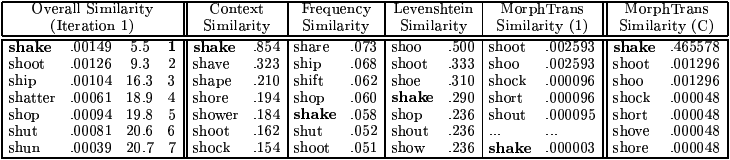
\includegraphics[scale=0.75]{yAw_table.png}
\caption{Candidate lemmas of the word \e{shook}. Source: \citep{yarowsky00}}
\label{table:yarowsky_table}
\end{table}

However, with highly inflected languages and other parts-of-speech than verbs, using this approach may be problematic. First, the context similarity measure assumes that inflections of the same lemma occur in similar context. Which works well with English verbs, as they have the same subcategorisation requirements in the past and in the present tense. On the other hand, if we consider Czech nouns, their accompanying adjectives exhibit agreement in case and number and therefore will be in a different form for differently inflected nouns (e.g. \e{zelená tráva} `green grass' (sg. nom.) vs. \e{zelenou trávou} (sg. ins.)).

Second, providing a list of all parts-of-speech and their canonical suffixes for languages with rich inflection would be more labour intensive as there can be hundreds or thousands of tags in the given language and less helpful, as there is great suffix homonymy in such languages. For example, \cite{feldman-hana-2010-rodopi} illustrate the homonymy of Czech using the suffix \e{a}, which has ``about 19 different meanings.'' (See Table \ref{table:ambiguity-a}) 

\begin{table}[h]
\begin{center}
\begin{tabular}{llll}

%
\toprule
\bf Form      & \bf Lemma    & \bf Gloss  & \bf Category                \\ 
\midrule
m\v{e}st-a    & m\v{e}sto    & town      & noun neuter sg gen           \\
          &          &                   & noun neuter pl nom (voc)     \\
          &          &                   & noun neuter pl acc           \\
t\'{e}m-a     & t\'{e}ma     & theme     & noun neuter sg nom (voc)     \\
          &          &                   & noun neuter sg acc           \\
\v{z}en-a     & \v{z}ena     & woman     & noun feminine sg nom            \\
p\'{a}n-a     & p\'{a}n      & man       & noun masculine anim sg gen      \\
          &          &                   & noun masculine anim sg acc      \\
ostrov-a  & ostrov   & island            & noun masculine inanim sg gen    \\
p\v{r}edsed-a & p\v{r}edseda & president & noun masculine anim sg nom      \\
vid\v{e}-l-a  & vid\v{e}t    & see       & verb past feminine sg           \\
          &          &                   & verb past neuter pl          \\
vid\v{e}-n-a  &          &               & verb passive feminine sg        \\
          &          &                   & verb passive neuter pl       \\
vid-a     &          &                   & verb transgressive masculine sg \\
dv-a      & dv-a     & two               & numeral masculine sg nom        \\
          &          &                   & numeral masculine sg acc        \\
\bottomrule
\end{tabular}
\end{center}
\caption{\label{table:ambiguity-a}Homonymy of the \e{a} ending in Czech (from \cite{feldman-hana-2010-rodopi})}
\end{table}

\subsection{Extended MorphTrans model as a supervised learner}
\cite{wicentowski04} extends the probabilistic model developed in \citep{yarowsky00} to handle prefixation and stem-internal vowel change. The extended model is called the WordFrame (WF) and it is used for supervised learning with training data in the form of \emph{$<$inflection, lemma$>$} pair list. Optional resources are a prefix list and a suffix list. Inflection is modelled as 5 possible transformations of the lemma: 
\begin{enumerate}
\item Adding a prefix $\psi_p'$ from the prefix list.
\item Point-of-prefixation stem change $\delta_p' \rightarrow \delta_p$
\item Stem internal vowel change $\delta_v' \rightarrow \delta_v$. $\delta_v'$ and $\delta_v$ may contain more than one vowel, but they must be both non-empty or both empty.
\item Point-of-suffixation stem change $\delta_s' \rightarrow \delta_s$
\item Removing a canonical suffix (e.g. infinitival ending for verbs) $\psi_s$ and adding a suffix $\psi_s'$ from the suffix list.
\end{enumerate}

\noindent Table \ref{table:wordframe} shows differences between the MorphTrans and the WordFrame model on the example of \e{kept} $\rightarrow$ \e{keep} transformation. The WordFrame is capable of capturing the stem internal change \e{e} $\rightarrow$ \e{ee}. Such rule is a better generalisation than the stem final change \e{p} $\rightarrow$ \e{ep}, for example it would work for \e{met} $\rightarrow$ \e{meet}.
\begin{table}[h]
\begin{center}
\begin{tabular}{llllllll}
\toprule
& $\psi_p'$    & $\delta_p' \rightarrow \delta_p$ & $\gamma_p$ & $\delta_v' \rightarrow \delta_v$ & $\gamma_s$ & $\delta_s' \rightarrow \delta_s$ & $\psi_s' \rightarrow \psi_s$     \\ 
\midrule
MorphTrans & N/A & N/A & N/A & N/A & ke & p $ \rightarrow$ ep & t $ \rightarrow \lambda$ \\
WordFrame & & & k &  e $\rightarrow$ ee & p &  & t $\rightarrow \lambda$\\
\bottomrule
\end{tabular}
\end{center}
\caption{\label{table:wordframe} Mapping \e{kept} $\rightarrow$ \e{keep} analysed by MorpTrans and WordFrame models. Source: \cite{wicentowski04}}
\end{table}

As a whole, inflection is a transformation $\delta_p \gamma_p \delta_v \gamma_s \delta_s \psi_s \rightarrow \psi_p' \delta_p' \gamma_p \delta_v' \gamma_s \delta_s' \psi_s'$ where ($\gamma_p \delta_v \gamma_s$, $\gamma_p \delta_v' \gamma_s$) is the \emph{WordFrame}, the longest common substring with at most one vowel change. Division of the training pairs into the subparts is done deterministically by:
\begin{enumerate}
\item Removing the longest matching prefix and suffix present in the affix lists from the inflection and a canonical prefix from the stem.
\item Finding the WordFrame.
\item Remaining strings on the left and right from the WF are considered $\delta_p/\delta_p'$ and $\delta_s/\delta_s'$.
\end{enumerate}

Analysis of an unseen inflection is done probabilistically by finding the lemma maximising \[P(\delta_p \gamma_p \delta_v \gamma_s \delta_s |\delta_p' \gamma_p \delta_v' \gamma_s \delta_s') = P(\delta_v' \rightarrow \delta_v, \delta_p' \rightarrow \delta_p, \delta_s' \rightarrow \delta_s|\delta_p' \gamma_p \delta_v' \gamma_s \delta_s')\] 
Point-of-suffixation change probability $P(\delta_s' \rightarrow \delta_s|\delta_p' \gamma_p \delta_v' \gamma_s \delta_s')$ is taken from a hierarchically smoothed suffix trie created in the training phase. $P(\delta_p' \rightarrow \delta_p|\delta_p' \gamma_p \delta_v' \gamma_s )$ is retrieved from an analogous prefix trie and the vowel change probability is estimated without regard on the local context (by $P(\delta_v|\delta_v')$).

The approach was tested on inflected verb forms in 32 languages, including Czech, with very good results. The size of the training data ranged from 9 lemmas and 201 inflections for Greek to 5715 lemmas and 23786 inflections for Czech.

\section{Automatic lexicon acquisition for provided pa\-ra\-digms}
The resource-light system by \cite{feldman-hana-2010-rodopi} uses manually specified pa\-ra\-digms as an input. The paradigms are specified by suffixes and point-of-affixation stem change rules. For each word in the corpus, possible paradigms are found and only the ones supported by the highest number of forms-tokens and/or form-types are retained.

\section{Semi-supervised systems using human elicitation}
\cite{oflazer01} describe a framework for creating morphological analysers of under-resourced languages. The framework makes use of direct human supervision in combination with machine learning in an iterative process. 

Input required from a human is a definition of paradigms. A paradigm is a set of words with (almost) the same inflectional behaviour. Each paradigm contains a primary example, optional secondary examples and a lexicon. An example is defined by its \emph{citation form} (the form one would look for in a dictionary) and inflected forms together with their morphological categories. The primary example must provide inflected forms for all values of relevant categories. This is not required for the secondary examples, which may be used to show irregularities for specific category combinations. A paradigm's lexicon contains citation forms of words which (presumably) belong to the paradigm.

After paradigm definition, the examples are automatically segmented in\-to stem and affixes. (Settings described in the paper allow at most one prefix and one suffix for a stem.) All string-prefixes (substrings beginning with the first letter) of a citation form (CF) are considered candidates for the stem. The candidate minimising the sum of  edit distances to all the inflected forms is chosen as a stem $s$. Then for each inflected form (IF), the projection of the stem is found (a substring with minimal edit distance to $s$). The remaining strings at the start and the end of the IF are considered prefix/suffix. The resulting segmentation is \emph{(prefix) + CF + (suffix)}. (The citation form is used instead of the stem.)

Segmented lexical forms are then aligned to the surface form as in the example (p. 71):
\begin{center}
\texttt{un + happy + est \hspace{10pt}  shop0 + ed\\
un 0 happi 0 est \hspace{10pt} shopp 0 ed}
\end{center} 
Alignment has 3 constraints : \begin{quote}
(i) a + in the segmented lexical form is always aligned with an empty string on the surface
side, notated by 0; (ii) a consonant on one side is always aligned with a consonant or 0 on the other side, and likewise for vowels; (iii) the alignment must correspond to the minimum edit distance between the original lexical and surface forms. (pp. 70 -- 71)
\end{quote}
Aligned pairs are used by a transformation based learner to learn context-based rewrite rules which transform the lexical forms into the surface forms. The rules are in form \texttt{u -> v || lc \_ rc}, where \texttt{u} is the symbol in the lexical form, \texttt{v} is the symbol in the surface form,  \texttt{lc} and  \texttt{rc} regular expressions describing left/right context of a limited length. For the previous examples, one can get rules like:
\begin{quote}
\begin{flushleft}
\texttt{y -> i || p \_ \\ 
y -> i || p \_ + e\\
y -> i || p \_ + e s \\ 
+ -> 0 || \# u n \_ h a p\\}
\end{flushleft}
\end{quote}
(p. 71), where \# denotes a word boundary, which may be used in context definition as well. The system allows assigning categories to characters and creation of more general rules by using categories in context definitions. In the presented implementation, characters are marked as consonants or vowels and for each rule, its generalised versions is generated. For example, the rule \texttt{0 -> p || p \_ + e} (p. 72) can be generalised by 3 different rules: \begin{quote}
\begin{flushleft}
\texttt{0 -> p || CONSONANT \_ + e}\\
\texttt{0 -> p || p + \_ VOWEL}\\
\texttt{0 -> p || CONSONANT \_ + VOWEL}\\
\end{flushleft}
\end{quote}
The same rule is often generated from more than one example. Number of such examples for a rule is called rule's \emph{promise}.

Rule selection is done iteratively by selecting the best rule and applying it to the list of lexical forms. Rules are sorted according to their promise, with the exception of the segmentation rules (\texttt{+ -> 0}), which are put to the bottom of the list. (The morpheme boundary is an important context for most of the rules and should not be removed prematurely.) The topmost rule, which does not cause errors (its application does not make any lexical form to be more distant from its corresponding surface form) is selected and applied to the lexical forms. The process is iterated until all the lexical forms are transformed to their corresponding surface forms.  

Using XRCE finite-state tools, the selected rules are compiled together with the lexicon to a finite-state transducer for the paradigm. The tools can be used for testing the analyser and finding where it makes mistakes. It is possible to generate all inflected forms for a citation form or all forms with one value of a category. 

When the analysers for paradigms are unioned to create the final analyser, a more elaborate method of testing is used. An error-tolerant finite-state recognizer engine is employed to find candidates for fixing -- words in a corpus which are not accepted by the analyser, but close to an accepted form. Then the human may adjust the system by adding more examples in an attempt to fix the errors and next iteration of learning is started.


\chapter{Paramor}\label{chapter:paramor}
In this chapter, I will describe Paramor, the system I have selected to build upon in this thesis. Paramor was introduced by Christian Monson in his PhD thesis \citep{monson09}. Its goal is unsupervised discovery of inflectional paradigms and using them for morpheme segmentation. 

To model partial paradigms, Monson uses \emph{schemes}. A scheme is defined by a set of candidate suffixes (c-suffixes, see Section \ref{sec:paramor_init}). The set of candidate stems (c-stems) adherent to a scheme is obtained deterministically by selecting all c-stems which can form a word (present in the corpus) with each of the scheme's c-suffixes. This is the main difference between schemes and Goldsmith's signatures, where each stem can be assigned only to a single signature.

Definition of schemes implies that with adding more c-suffixes into a scheme, number of c-stems can only drop or stay the same. Schemes form a lattice when we consider partial ordering defined by c-suffix set inclusion. Figure \ref{fig:scheme_lattice}, taken from \citep{monson09}, illustrates a part of a scheme lattice for an English corpus. The highlighted scheme, (\e{0, ed, ing, s}) has 106 adherent c-stems. Adding the c-suffix \e{ly} causes a drop to only 4 c-stems, while removing the c-suffix \e{s} increases the c-stem count to 201.

\begin{figure}[p]
\centering
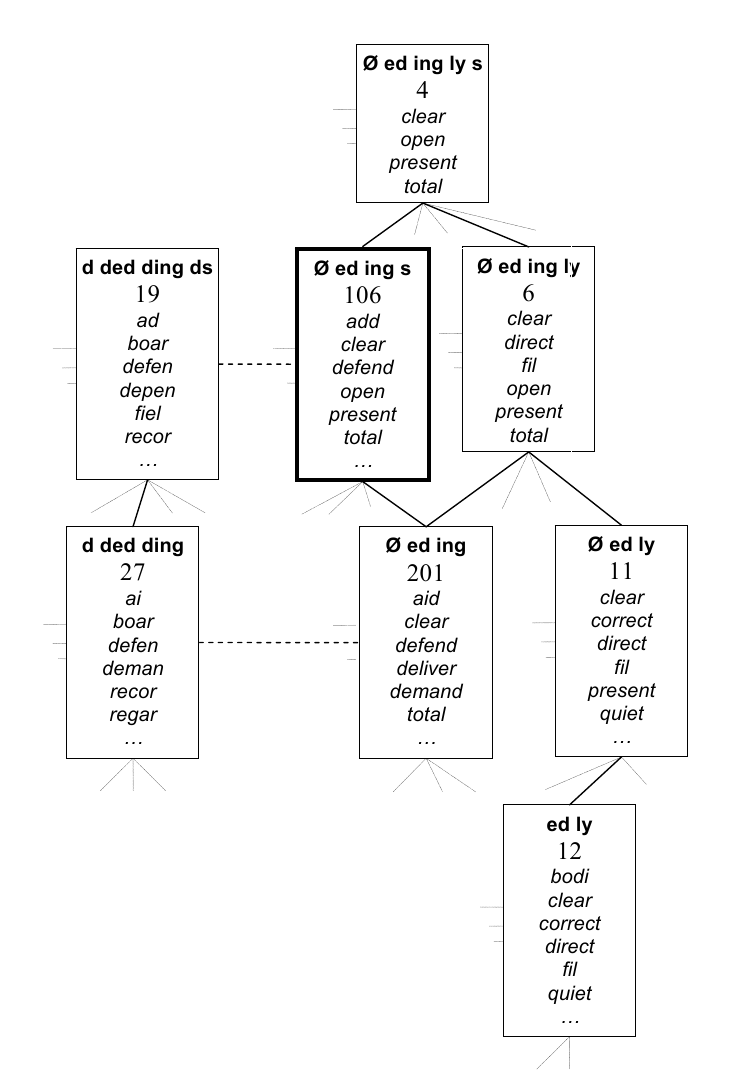
\includegraphics[scale=0.6]{schemeLattice.png}
\caption{Example part of a scheme lattice. Source: \citep{monson09}}
\label{fig:scheme_lattice}
\end{figure}

\section{Steps in Paramor's pipeline}

\subsection{Initialisation}\label{sec:paramor_init}
In the first step, sets of candidate stems (c-stems) and candidate suffixes (c-suffixes) are populated by considering every possible split into stem and suffix for every word in the corpus.

\subsection{Bottom-up Search}

Next phase of the algorithm performs a bottom-up search in the scheme lattice, starting with schemes containing exactly one c-suffix. For each of them, Paramor ascends the lattice, adding one c-suffix at a time until a stopping criterion is met. C-suffix selected for adding is the one with the biggest c-stem ratio. C-stem ratio is the ratio between the number of c-stems in the candidate higher-level scheme and the current scheme. When the highest possible c-stem ratio falls under 0.25, search stops. 

For illustration, let's use the lattice from Figure \ref{fig:scheme_lattice} and assume that the search has reached the (\e{0, ed, ing}) scheme, which has 201 adherent c-stems. There are two schemes the search can continue to: (\e{0, ed, ing, ly}) with 6 c-stems and (\e{0, ed, ing, s}) with 106 c-stems. The algorithm selects the scheme with the highest number of c-stems -- (\e{0, ed, ing, s}) and checks whether the c-stem ratio is above 0.25. The ratio is 106 / 201 = 0.53 and the search moves to the highlighted scheme. Then there is only one possibility to continue: (\e{0, ed, ing, s, ly}) with only 4 c-stems, which is rejected due to the c-stem ratio 4 / 106 = 0.04.

\subsection{Scheme Clustering}

Resulting schemes are then subjected to agglomerative bottom-up clustering. To determine proximity of two clusters, sets of (word) types generated by the clusters are measured by cosine similarity.\footnote{proximity($X$,$Y$) = $\frac{|X \cap Y|}{\sqrt{|X||Y|}}$} Cluster generates a set of types which is union of sets generated by the schemes it contains. In order to be merged, clusters must satisfy some conditions, e.g. for any two suffixes in the cluster, there must be a stem in the cluster which can combine with both of them.

\subsection{Pruning}

After clustering phase, there are still too many clusters remaining and pruning is necessary. In the first pruning step, clusters which generate only small number of types are discarded. Then Paramor tries to identify clusters modelling incorrect morpheme boundary in a Harrisian fashion by using letter entropy.

\subsection{Segmentation}

Remaining clusters can be used to segment the `training' corpus or a previously unseen text. For every word in the text, every possible division between stem $t$ and suffix $f$ is examined. If there is a cluster containing $f$ and another suffix $f'$ such that $t.f'$ is a word from the training corpus or the text, Paramor declares morpheme boundary between $t$ and $f$. In this way, more than one morpheme boundary may be found in single word. For example, the algorithm analyses \e{talks} as \e{talk} + \e{s} using the scheme cluster (0, \e{s}, \e{ing}) if \e{talk} or \e{talking} is found in the corpus. 

\section{Results and discussion}

Paramor took part in Morpho Challenge 2008\footnote{\url{http://research.ics.tkk.fi/events/morphochallenge2008/}} with excellent results, especially when combined with Morfessor. Both algorithms achieved precision higher than recall, so a natural idea was to design a combined analyser, returning the union of Paramor's and Morfessor's hypothesised morpheme boundaries. The combined analyser outperformed the other competitors in all 5 of the test languages.\footnote{In Competition 1, which directly evaluated placing of the morpheme boundaries. In Competition 2, which applied the analyses in an IR system, Paramor+Morfessor won in 1 of the 3 languages.} 

Useful feature of Paramor is that besides being able to segment texts, it outputs the scheme clusters in a human-readable way. Examining the clusters may help getting basic insight into grammatical structure of an unknown language.

A certain disadvantage of Paramor is that it does not handle the phonological/gra\-phe\-mic changes triggered by the affixation, such as the ones shown in Table \ref{table:matka}. Thus, it faces a similar problem as the engineering approach to morphology (see Section \ref{sec:engineer}) -- the need to create much larger number of paradigms. Unlike in the engineering approach, where paradigms are entered manually, Paramor  must find the evidence for the paradigms in the corpus. The richer the inflection of the language is, the more problematic sparsity becomes. An attempt to improve the algorithm by working with allomorphic variants of stems is presented in the following chapter.

\chapter{Modifications of Paramor}\label{chapter:modifications}

Modifications of Paramor were conducted with two motives: 
\begin{enumerate}
\item Create a semi-supervised system, using manually provided seed of inflected words divided into stems and suffixes.

\item Take into account basic allomorphy of stems.
\end{enumerate} 
\noindent The modifications were realised by directly changing Paramor's code, rather than by pre-/post-processing. Figure \ref{fig:overview} shows phases of Paramor on the left with dashed boxes representing my alterations.

\begin{figure}
\begin{center}
\newcommand{\paramorXA}{1.5}
\newcommand{\paramorXB}{7.8}

\newcommand{\parStepXA}{1.8}
\newcommand{\parStepXB}{7.5}

\newcommand{\seedXA}{9.2}
\newcommand{\seedXB}{10.9}
\newcommand{\seedXMid}{10.0}
\newcommand{\seedXCorn}{10.5}

\newcommand{\autoseedXA}{12.2}
\newcommand{\autoseedXB}{16.0}
\newcommand{\autoseedXMid}{14.1}
\newcommand{\autoseedXCorn}{15.5}

\newcommand{\clusteringXA}{8.5}
\newcommand{\clusteringXB}{11.5}
\newcommand{\clusteringXMid}{10.0}


\ifx\du\undefined
  \newlength{\du}
\fi
\setlength{\du}{15\unitlength}
{\footnotesize
\begin{tikzpicture}
\pgftransformxscale{1.000000}
\pgftransformyscale{-1.000000}
\pgfsetlinewidth{0.075000\du}
\pgfsetdash{}{0pt}
\pgfsetdash{}{0pt}
\pgfsetbuttcap
\pgfsetmiterjoin
\pgfsetlinewidth{0.075000\du}
\pgfsetbuttcap
\pgfsetmiterjoin
\pgfsetdash{}{0pt}
\draw (3.664332\du,1.100000\du)--(5.130582\du,1.100000\du)--(5.619332\du,1.588750\du)--(5.619332\du,3.043750\du)--(3.664332\du,3.043750\du)--cycle;
\pgfsetbuttcap
\pgfsetmiterjoin
\pgfsetdash{}{0pt}
\draw (5.130582\du,1.100000\du)--(5.130582\du,1.588750\du)--(5.619332\du,1.588750\du)--(5.619332\du,1.588750\du);
\pgfsetlinewidth{0.075000\du}
\pgfsetdash{}{0pt}
\pgfsetdash{}{0pt}
\pgfsetbuttcap
\pgfsetmiterjoin
\pgfsetlinewidth{0.075000\du}
\pgfsetbuttcap
\pgfsetmiterjoin
\pgfsetdash{}{0pt}
%Manual seed box
\draw (\seedXA\du,9.410000\du)--(\seedXCorn\du,9.410000\du)--(\seedXB\du,9.810000\du)--(\seedXB\du,11.410000\du)--(\seedXA\du,11.410000\du)--cycle;
\pgfsetbuttcap
\pgfsetmiterjoin
\pgfsetdash{}{0pt}
\draw (\seedXCorn\du,9.410000\du)--(\seedXCorn\du,9.810000\du)--(\seedXB\du,9.810000\du)--(\seedXB\du,9.810000\du);

%Auto seed box
\draw (\autoseedXA\du,9.410000\du)--(\autoseedXB\du,9.410000\du)--(\autoseedXB\du,11.0\du)--(\autoseedXA\du,11.0\du)--cycle;

%Paradigms from Paramor box
\draw (\autoseedXA\du,12.410000\du)--(\autoseedXB\du,12.410000\du)--(\autoseedXB\du,14.0000\du)--(\autoseedXA\du,14.0000\du)--cycle;

% Paramor small box
\draw (\autoseedXA\du,15.410000\du)--(\autoseedXB\du,15.410000\du)--(\autoseedXB\du,17.0000\du)--(\autoseedXA\du,17.0000\du)--cycle;

%paradigms1 box
%\draw (\clusteringXA\du,13.0000\du)--(\clusteringXB\du,13.0000\du)--(\clusteringXB\du,14.4000\du)--(\clusteringXA\du,14.4000\du)--cycle;

%Clustering box
%\draw (\clusteringXA\du,15.410000\du)--(\clusteringXB\du,15.410000\du)--(\clusteringXB\du,17.0000\du)--(\clusteringXA\du,17.0000\du)--cycle;

% Word clusters box
%x\draw (\clusteringXA\du,17.8200\du)--(\clusteringXB\du,17.8200\du)--(\clusteringXB\du,19.410\du)--(\clusteringXA\du,19.4100\du)--cycle;

\pgfsetlinewidth{0.075000\du}
\pgfsetdash{}{0pt}
\pgfsetdash{}{0pt}
\pgfsetmiterjoin
%whole Paramor box
\draw (\paramorXA\du,3.9\du)--(\paramorXA\du,14.3\du)--(\paramorXB\du,14.3\du)--(\paramorXB\du,3.9\du)--cycle;
%\node at (4.652188\du,6.075000\du){};

\pgfsetlinewidth{0.075000\du}
\pgfsetdash{}{0pt}
\pgfsetdash{}{0pt}
\pgfsetmiterjoin
%stem-suf map box
\draw (\parStepXA\du,4.955000\du)--(\parStepXA\du,6.855000\du)--(\parStepXB\du,6.855000\du)--(\parStepXB\du,4.955000\du)--cycle;
\node at (4.652188\du,6.075000\du){};
\pgfsetlinewidth{0.075000\du}
\pgfsetdash{}{0pt}
\pgfsetdash{}{0pt}
\pgfsetmiterjoin
%Bottom-up search box
\draw (\parStepXA\du,7.850000\du)--(\parStepXA\du,10.150000\du)--(\parStepXB\du,10.150000\du)--(\parStepXB\du,7.850000\du)--cycle;
\node at (4.652188\du,9.170000\du){};
\pgfsetlinewidth{0.075000\du}
\pgfsetdash{}{0pt}
\pgfsetdash{}{0pt}
\pgfsetmiterjoin
%Scheme clustering box
\draw (\parStepXA\du,11.460000\du)--(\parStepXA\du,13.850000\du)--(\parStepXB\du,13.850000\du)--(\parStepXB\du,11.460000\du)--cycle;
\node at (4.652188\du,12.825000\du){};
\pgfsetlinewidth{0.075000\du}
\pgfsetdash{}{0pt}
\pgfsetdash{}{0pt}
\pgfsetmiterjoin
%Segmentation box
\draw (\parStepXA\du,15.270000\du)--(\parStepXA\du,17.170000\du)--(\parStepXB\du,17.170000\du)--(\parStepXB\du,15.270000\du)--cycle;
%\node at (4.652188\du,16.390000\du){Segmentation};
\node at (4.652188\du,16.390000\du){Word clusters};
\pgfsetlinewidth{0.075000\du}
\pgfsetdash{}{0pt}
\pgfsetdash{}{0pt}
\pgfsetmiterjoin
\draw (9.145000\du,4.955000\du)--(9.145000\du,6.855000\du)--(14.570000\du,6.855000\du)--(14.570000\du,4.955000\du)--cycle;
\node at (11.857500\du,6.075000\du){};
\node at (4.641832\du,2.066875\du){Corpus};
\pgfsetlinewidth{0.075000\du}
\pgfsetdash{}{0pt}
\pgfsetdash{}{0pt}
\pgfsetbuttcap
{
\pgfsetarrowsend{to}
\draw (4.641832\du,3.043750\du)--(4.647809\du,4.906542\du);
}
\pgfsetlinewidth{0.075000\du}
\pgfsetdash{}{0pt}
\pgfsetdash{}{0pt}
\pgfsetbuttcap
{
\pgfsetarrowsend{to}
\draw (4.652188\du,6.855000\du)--(4.652188\du,7.850000\du);
}
\pgfsetlinewidth{0.075000\du}
\pgfsetdash{}{0pt}
\pgfsetdash{}{0pt}
\pgfsetbuttcap
{
\pgfsetarrowsend{to}
\draw (4.652188\du,10.150000\du)--(4.652188\du,11.460000\du);
}
\pgfsetlinewidth{0.075000\du}
\pgfsetdash{}{0pt}
\pgfsetdash{}{0pt}
\pgfsetbuttcap
{
\pgfsetarrowsend{to}
\draw (4.652188\du,13.850000\du)--(4.652188\du,15.270000\du);
}
%text labels
\node at (\seedXMid\du,10.1\du){Man.};
\node at (\seedXMid\du,10.8\du){seed};
%\node at (\seedXMid\du,11.9\du){Manual seed};
\node at (\autoseedXMid\du,10.2\du){Autoseed};
\node at (\autoseedXMid\du,13.2\du){Paradigms};
\node at (\autoseedXMid\du,16.2\du){Paramor};
%\node at (\clusteringXMid\du,13.7\du){Paradigms};
%\node at (\clusteringXMid\du,16.2\du){Clustering};
%\node at (\clusteringXMid\du,18.4\du){Word};
%\node at (\clusteringXMid\du,18.9\du){clusters};
\pgfsetlinewidth{0.075000\du}
\pgfsetdash{}{0pt}
\pgfsetdash{}{0pt}
\pgfsetbuttcap
{
\pgfsetarrowsend{to}
\draw (9.145000\du,5.905000\du)--(7.002188\du,6.232600\du);
}
\pgfsetlinewidth{0.075000\du}
\pgfsetdash{}{0pt}
\pgfsetdash{}{0pt}
\pgfsetbuttcap
{
\pgfsetarrowsend{to}
\draw (\seedXA\du,10.410000\du)--(7.102188\du,9.351300\du);
}
\pgfsetlinewidth{0.075000\du}
\pgfsetdash{}{0pt}
\pgfsetdash{}{0pt}
\pgfsetbuttcap
{
\pgfsetarrowsend{to}
\draw (\seedXA\du,10.410000\du)--(7.113750\du,13.051300\du);
}
\pgfsetlinewidth{0.075000\du}
\pgfsetdash{}{0pt}
\pgfsetdash{}{0pt}
%man. seed -> rule generation
\pgfsetbuttcap
{
\pgfsetarrowsend{to}
\draw (10.0\du,9.410000\du)--(11.857500\du,6.855000\du);
}
\node[anchor=west] at (8.045000\du,11.447500\du){};

%auto seed -> rule generation
\pgfsetbuttcap
{
\pgfsetarrowsend{to}
\draw (\autoseedXMid\du,9.410000\du)--(11.857500\du,6.855000\du);
}

%paradigms -> auto seed
\pgfsetbuttcap
{
\pgfsetarrowsend{to}
\draw (\autoseedXMid\du,12.4\du)--(\autoseedXMid\du,11.0\du);
}

%paramor small-> paradigms
\pgfsetbuttcap
{
\pgfsetarrowsend{to}
\draw (\autoseedXMid\du,15.4\du)--(\autoseedXMid\du,14.0\du);
}

%paramor small-> paradigms
%\pgfsetbuttcap
%{
%\pgfsetarrowsend{to}
%\draw (\parStepXB\du,13.5\du)--(\clusteringXA\du,13.5\du);
%}

%paradigms1-> clustering
%\pgfsetbuttcap
%{
%\pgfsetarrowsend{to}
%\draw (\clusteringXMid\du,14.4\du)--(\clusteringXMid\du,15.4\du);
%}
%
%%clustering-> clusters
%\pgfsetbuttcap
%{
%\pgfsetarrowsend{to}
%\draw (\clusteringXMid\du,17.00\du)--(\clusteringXMid\du,17.8\du);
%}

\pgfsetlinewidth{0.050000\du}
\pgfsetdash{{2pt}{2pt}}{0pt}

\pgfsetmiterjoin
\draw (2.302188\du,5.841300\du)--(2.302188\du,6.623900\du)--(7.002188\du,6.623900\du)--(7.002188\du,5.841300\du)--cycle;
\node at (4.652188\du,6.348800\du){deep stems};

\pgfsetlinewidth{0.050000\du}
\pgfsetdash{{2pt}{2pt}}{0pt}
\pgfsetmiterjoin
\draw (2.202188\du,8.718700\du)--(2.202188\du,9.983900\du)--(7.102188\du,9.983900\du)--(7.102188\du,8.718700\du)--cycle;
\node at (4.652188\du,9.226200\du){more starting};
\node at (4.652188\du,9.708800\du){schemes};
\pgfsetlinewidth{0.050000\du}
\pgfsetdash{{2pt}{2pt}}{0pt}
\pgfsetmiterjoin
\draw (2.190625\du,12.418700\du)--(2.190625\du,13.683900\du)--(7.113750\du,13.683900\du)--(7.113750\du,12.418700\du)--cycle;
\node at (4.652188\du,12.926200\du){keep some clusters };
\node at (4.652188\du,13.408800\du){from discarding};
\node[anchor=west] at (2.30\du,5.500000\du){Stem-suffix map};
\node[anchor=west] at (2.3000\du,8.425000\du){Bottom-up search};
\node[anchor=west] at (2.30\du,12.0000\du){Scheme clustering};
\node[anchor=west] at (9.8000\du,5.90000\du){Rule induction};

\node[anchor=west] at (1.30\du,4.300000\du){Paramor};


\end{tikzpicture}
}

\end{center}
\caption{Altered Paramor's pipeline}
\label{fig:overview}
\end{figure}

In the bottom-up search phase and the scheme cluster filtering phase, the manually provided examples of valid suffixes and their grouping to sub-paradigms are used to steer Paramor towards creating more adequate schemes and scheme clusters. 
If the seed contains allomorphic stems, they are used to induce simple stem rewrite rules. Using these rules, part of the allomorphic stems in the corpus can be discovered, which helps to find more complete schemes.

\section{Scheme seeding}

\noindent
The manual seed contains a simple list of inflected words with marked morpheme boundary. English inflections
\begin{quote}
\e{talk, talks, talked, talking}\\
\e{stop, stops, stopped, stopping}\\
\e{chat, chats, chatted, chatting}
\end{quote}

\noindent
would be captured as:

\begin{quote}
\e{talk, stop/stopp, chat/chatt +  0, s / ed, ing}
\end{quote}

\noindent
The format of the seed and the seeds used in the evaluation are described in the appendix \ref{chapter:seeds}. The data are used to enhance Paramor's accuracy in discovering the correct schemes and scheme clusters in the following way:
\begin{enumerate}
\item In the bottom-up search, Paramor starts with single-affix schemes. I added a 2-affix scheme to the initial scheme set for every suffix pair from the manual data belonging to the same inflection. Note that one cannot simply add a scheme containing all the suffixes of the whole paradigm as many of the forms will not be present in the corpus.

Thus, for \e{talk + 0, s, ed, ing}, one would add the following schemes to the initial scheme set: \e{(0, s), (0, ed), (0, ing), (s, ed), (s, ing), (ed, ing)}

\item Scheme clusters containing suffixes similar to some of the manually entered suffix sets are protected from the second phase of the cluster pruning. More precisely, a cluster is protected if at least half of its schemes share at least two suffixes with a particular manual suffix set.

For example, a scheme cluster with suffixes (\e{í, ích, ímu, ími, ě, ím, ího, ictví}) induced from a Czech corpus was protected from discarding because it contained the suffixes (\e{í, ím, ího, ímu}), present in one of the examples in the Czech seed -- (\e{letn + í, ím, ího, ímu}) `summer' masc. sg. adjective, nom, ins, gen/acc, dat respectively.

\end{enumerate}

\section{Allomorphy}

Paramor ignores allomorphy completely (and so do Linguistica and Mofessor). There are at least two reasons to handle allomorphy. First, linguistically, it  makes  more  sense  to  analyse  \e{winning}  as  \e{win+ing} than as  \e{winn+ing} or \e{win+ning}. For  many  applications, such as information retrieval, it is helpful to know that two morphs are variants of the same morpheme.
%
Second, ignoring allomorphy makes the data appear more complicated and noisier than they actually are. Thus, the process of learning morpheme boundaries or paradigms is harder and less successful.

This latter problem might manifest itself in Paramor's bottom-up search phase: a linguistically correct suffix triggering a stem change might be discarded, because Paramor would not consider stem allomorphs to be variants of the same stem and c-stem ratio may drop significantly. Further more, incorrect c-suffixes may be selected.

For example, suppose there are 5 English verbs in the corpus: \emph{talk, hop, stop, knit, chat}, together with their \emph{-s} (\emph{talks, hops, stops, knits, chats}) and \emph{-ing} (\emph{talking, hopping, stopping, knitting, chatting}) forms. Let's already have a scheme \{\emph{0, s}\} with 5 stems. Adding \emph{ing} would decrease the number of stems to 1, leaving only \emph{talk} in the scheme. C-stem ratio would be 0.2 and \emph{ing} would not be accepted. Moreover, incorrect c-suffixes as \emph{ping} and \emph{ting} have c-stem ratio 0.4 and may be accepted.

%\subsubsection{Stem change rule induction}

However, for most languages the full specification of rules constraining allomorphy is not available, or at least is not precise enough. Therefore, I automatically induce a limited number of simple rules from the seed examples and/or from the scheme clusters obtained from the previous run of algorithm. Such rules both over- and undergenerate, but nevertheless they do improve the accuracy of the whole system. For languages, where formally specified allomorphic rules are available, they can be used directly along the lines of
\cite{tepper10,tepper-xia-2008}, see Section \ref{section:semisup_morfessor}.
%
Currently the system  considers only stem final changes, namely vowel epenthesis (\eg
\e{matk+a} -- \e{matek+0}) and alternation of the final consonant (\eg \e{matk+a} -- \e{matc+e}). %The extension to other other processes such as root vowel change (\eg English \e{foot -- feet}) is quite straightforward, but we leave with for future work.


\subsection{Stem change rule induction and application}
Formally, the process can be described as follows.
From every pair of stem allomorphs in the seed, $a\delta_1, a\delta_2$, where $a$ is their longest common initial substring\footnote{should $\delta_1$ or $\delta_2$ be 0, one final character is removed from $a$ and prepended to $\delta_1$ and $\delta_2$} 
with suffix sets $F_1$, $F_2$  a correspondence rule is generated $*\delta_1 \leftrightarrow *\delta_2$ / $(F_1, F_2)$. A rule $*\delta_1 \leftrightarrow *\delta_2$ / $(F_1, F_2)$ is applicable on an unordered pair of c-stems {$x\delta_1$, $x\delta_2$} present in the corpus if:

\begin{enumerate}
\item C-suffix set of the c-stem $x\delta_1$ contains at least one of the suffixes from $F_1$ and contains no suffix from $F_2$.
\item C-suffix set of the c-stem $x\delta_2$ contains at least one of the suffixes from $F_2$ and contains no suffix from $F_1$.
\end{enumerate}

\noindent For example, from a seed entry 
\begin{quote}
\e{politik/politic + a, u, ovi, em, y, ů, ům / i, ích}
\end{quote}
the following rule is generated:
\begin{quote}
$*k \leftrightarrow *c$ / (\{\e{a, u, ovi, em, y, ů, ům}\}, \{\e{i, ích}\}) 
\end{quote}

The rules are used to generate underlying form of c-stems, which I call \emph{deep} stems.  I define relation $\leftrightarrow$ between two c-stems: $s_1 \leftrightarrow s_2$ iff there is a correspondence between $s_1$ and $s_2$ licensed by any rule. The deep stems then correspond to equivalence classes induced by the reflexive and transitive closure of $\leftrightarrow$.
%\noindent
%Formally, the process can be described as follows.
%From every pair of stem allomorphs in the manual input, $s\delta_1, s\delta_2$, where $s$ is their longest common initial substring,\footnote{should $\delta_1$ or $\delta_2$ be 0, one final character is removed from $s$ and prepended to $\delta_1$ and $\delta_2$} with suffix
%sets $f_1$, $f_2$ we generate a rule $*\delta_1 \rightarrow *\delta_2$ / $(f_1, f_2)$ and also a reverse rule $*\delta_2 \rightarrow *\delta_1$ / $(f_2, f_1)$. Notation $*\delta_1 \rightarrow *\delta_2$ / $(f_1, f_2)$ means ``transform a stem $x\delta_1$ into $x\delta_2$ if following conditions hold:''
%
%\begin{enumerate}
%\item $x\delta_2$ is a c-stem present in the corpus.
%\item C-suffix set $f^x_1$ (from the corpus) of the c-stem $x\delta_1$ contains at least one of the suffixes from $f_1$ and contains no suffix from $f_2$.
%\item C-suffix set $f^x_2$ of the c-stem $x\delta_2$ contains at least one of the suffixes from $f_2$ and contains no suffix from $f_1$.
%\end{enumerate}
%
%\noindent
%Induced rules are applied after the initialisation phase. So-called \emph{deep} stems are generated from the c-stems. A deep stem is defined as a set of surface stems.
%
%To obtain a deep stem for a c-stem $t$, operation of \emph{expansion} is applied. Expansion works as a breadth-first search using a queue initialised with $t$ and keeping track of the set $D$ of already generated variants. While the queue is not empty, the first member is removed and its variants found by application of all the rules. (Result of applying a rule si non-empty only if the rule is applicable and its right hand side is present in the corpus.) Variants which haven't been generated so far are added to the back of the queue and to $D$. When the queue is emptied, $D$ becomes the deep stem associated with $t$ and all other members of $D$.
%
Bottom-up search and all the following phases of Paramor algorithm are then using the deep stems instead of the surface ones.

\subsection{Stem change rule induction from scheme clusters}\label{section:autoseed}

\noindent
In addition to deriving allomorphic rules from the manual seed, I also tested a heuristic for detecting stem allomorphy in the scheme clusters obtained from the previous run of the algorithm.
%
Stem allomorphy increases the sparsity problem and might prevent Paramor from finding complete paradigms. However, if the stem changes are systematic and frequent, Paramor does create the appropriate scheme clusters, although it considers the changing part of the stem to be a part of suffixes.

As an example, consider again the declension of the Czech word \gloss{matka}{mother} in Table \ref{table:matka}. Paramor's scheme cluster with suffixes \{\emph{ce, ek, ka, kami, kou, ku, ky, kách, kám}\} has correctly discovered 9 of the 10 paradigm's suffixes,\footnote{Except for vocative case singular, which is rarely used.} but fused together with parts of the stem. (Practically discovering the ``engineering'' paradigm from Table \ref{table:matka_eng})
Presence of such scheme cluster in the Paramor's output is a hint that there may be a \e{c/k} alternation and epenthesis in the language. The heuristic presented in this section tries to find scheme clusters with similar characteristics as the \{\emph{ce, ek, ka, ...}\} cluster and create stem variants by moving the morpheme boundary.

In the first phase, each scheme cluster with a c-suffix set $F$ is tested by the following procedure:
\begin{enumerate}
\item If $F$ contains a c-suffix without a consonant, return \emph{false}.
\item $c_c$ = count of unique left-most consonants found in the c-suffixes in $F$.
\item If $c_c > 2$ return \emph{false}. If $c_c$ = 1 and $F$ doesn't contain any c-suffix starting with a vowel, return \emph{false}.
\item Return \emph{true}.
\end{enumerate}
If a scheme cluster passes this test, each of its stems' subparadigms is examined. Subparadigm for stem $s$ consists of $s$ and $F_s$ -- all the c-suffixes from $F$ with which $s$ forms a word in the corpus. For example, let's have a stem $s = $ \emph{mat} with $F_s = $ \{\emph{ce, ek, ka, ku, ky}\}. Now, the morpheme boundary is shifted so that it is immediately to the right from the first consonant of the original c-suffixes. In the \e{matka} example, 3 stem variants emerge after the shift:\begin{quote}
\begin{flushleft}
\emph{matk} + \emph{a, u, y}\\
\emph{matc} + \emph{e}\\ 
\emph{matek} + \emph{0}\\
\end{flushleft}
\end{quote}
To reduce the amount of falsely detected phonological changes, each stem variant's suffix set is checked whether it contains at least one of the c-suffixes that Paramor has already discovered in other scheme clusters. If the condition holds, rules with the same syntax as the manual seed are created. For example, \begin{quote}\emph{matk / matc / matek} + \emph{a, u, y / e / 0}\end{quote} All generated rules are gathered in a file and can be used in the same way as the manual seed or just for the induction of phonological rules.

\subsubsection*{Automatically discovered rules for Czech}

The heuristic, when tested on scheme clusters generated by Paramor for a Czech corpus with 25k word types, was able to detect a number of phonological/graphemic changes. Examples of detected palatalisation are shown in Table \ref{table:autoseed_palat}. Table \ref{table:autoseed_epen} presents some of the detected cases of epenthesis.

\begin{table}[p]
\centering
\begin{tabular}{r@{\, $\rightarrow$ \,}l}
\toprule
%\bf Change & \bf Cost\\
%\midrule
\gloss{kni\textbf{h} + a}{book\subscr{nom.sg.}} & \gloss{kni\textbf{z} + e}{book\subscr{loc.sg.}}\\
\gloss{strán\textbf{k} + a}{page\subscr{nom.sg.}} & \gloss{strán\textbf{c} + e}{page\subscr{dat.sg.}}\\
\gloss{atmosfé\textbf{r} + a}{atmosphere\subscr{nom.sg.}} & \gloss{atmosfé\textbf{ř} + e}{atmosphere\subscr{loc.sg.}}\\
\gloss{umě\-le\textbf{c}  + ký}{artistic\subscr{nom.sg.}} & \gloss{uměle\textbf{č} + tí}{artistic\subscr{nom.pl.}}\\
\gloss{vojen\textbf{s}  + ký}{military\subscr{nom.sg.}} & \gloss{vojen\textbf{š} + tí}{military\subscr{nom.pl.}}\\
\bottomrule
\end{tabular}
\caption{\label{table:autoseed_palat} Examples of detected palatalisation.}
\end{table}

\begin{table}[p]
\centering
\begin{tabular}{r@{\, $\rightarrow$ \,}l}
\toprule
%\bf Change & \bf Cost\\
%\midrule
\gloss{volb + a}{choice\subscr{nom.sg.}} & \gloss{vol\textbf{e}b + 0}{choices\subscr{gen.pl.}}\\
\gloss{poplatk + y}{fees\subscr{nom.pl.}} & \gloss{poplat\textbf{e}k + 0}{fee\subscr{nom.sg.}}\\
\gloss{pohádk + y}{fairy tales\subscr{nom.pl.}} & \gloss{pohád\textbf{e}k + 0}{fairy tales\subscr{gen.pl.}}\\
\gloss{požadavk + ům}{requests\subscr{dat.pl.}} & \gloss{požadav\textbf{e}k + 0}{request\subscr{nom.sg.}}\\
\bottomrule
\end{tabular}
\caption{\label{table:autoseed_epen} Examples of detected epenthesis.}
\end{table}

\noindent There were also incorrect rules generated, for example \fromTo{poklesl + a}{poklesn + e}, which relates fem. past participle and 3p. sg. future forms of \gloss{poklesnout}{to decrease}. There is no alternation \fromTo{l}{n} in Czech and the Paramor's original analysis \e{pokles + la}, \e{pokles + ne} was correct.

\section{Rules for inflectional prefixes}\label{section:prefixes}
I have also enabled supplying a list of the inflectional prefixes of the given language to Paramor. This feature was tested on Czech, which has only two inflectional prefixes (negative prefix \e{ne} and superlative prefix \e{nej}). The decision which prefixes to consider inflectional and which not is to a certain degree an arbitrary decision (\eg it can be argued that \e{ne} is a clitic and not a prefix), therefore it makes sense to provide such information manually.


\chapter{Clustering Framework}\label{chapter:clustering}

The second software package developed for this thesis is a framework for bottom-up clustering. Although its primary purpose is creating and evaluating clusters of morphologically related words, it is general and allows clustering of any objects (not only strings) and using custom distance metrics. 

The bottom-up clustering algorithm is simple: At the beginning, one cluster is created for each object. Then, until the stopping criterion is met, the two clusters with the smallest distance between them are merged in each step. Stopping criteria supported by the framework are reaching a predefined number of clusters or the smallest distance between clusters growing above a given threshold. 

Once the distance measure between two objects is defined, there is a number of ways to define distance between clusters of objects. Currently, the framework supports 3 of them:
\begin{enumerate}
\item Nearest member. Distance between clusters A and B is defined as the \textbf{smallest} distance between a member of A and a member of B.
\item Furthest member. Distance between clusters A and B is defined as the \textbf{largest} distance between a member of A and a member of B.
\item Average distance. Distance between clusters A and B is defined as the \textbf{average} distance between a member of A and a member of B. 
\end{enumerate}

\section{Application to morphology}

To use the framework for creating clusters of morphologically related words, it is necessary to define a distance measure between two words. The framework contains 3 pre-built distance measure types. The first one is based on modified edit distance and the other two allow results of unsupervised learners to be used in the clustering. The measures are described below. Euclidean combination of any number of distances is also supported.

\subsection{Edit distance}
As the basic form of the edit distance, the framework contains the Levenshtein distance \citep{levenshtein66}, a distance recognising three basic operations on a string: deletion, insertion or substitution of a single character. By default, each operation has the same cost contributing to the overall distance. 

The distance metric can be customised by providing a cost matrix for substitution of characters. This matrix can, for example, represent the fact that some phonemes (represented by graphemes) share more phonological features than others. In such a case, it would make sense to decrease for example the cost of the \e{s/z} substitution. To design such matrix, one must have quite a detailed knowledge of given language's phonology and orthography. A more resource-light (but less linguistically adequate) approach would just decrease the distance between vowels and between characters differing only in a diacritic marks, such as \e{a/á} in Czech or \e{a/ä} in German.

Besides the customisable Levenshtein distance, the framework also contains its modification in which the cost of an operation linearly decreases with the position in the string where it occurs. This distance can serve as a very simple model of suffix-based morphology. 
In the experimental evaluation, I have used this distance in combination with the above-mentioned approach lowering the costs for diacritics adding/removing and vowel changes. Table \ref{table:edit_config} shows the concrete costs I have selected for use in the experiments.

\begin{table}[h]
\centering
\begin{tabular}{lr}
\toprule
\bf Change & \bf Cost\\
\midrule
vowel $ \leftrightarrow $ vowel 				& 0.7\\
with diacritic $ \leftrightarrow $ w/o diac.    & 0.5\\
other & 1.0\\
\bottomrule
\end{tabular}
\caption{\label{table:edit_config} Edit costs used in the experiments.}
\end{table}

\subsection{Segmentation distance}
To be able to employ morpheme segmentation algorithms such as Morfessor, I defined a string distance metric based on the words' morphemic segmentation. For a word with $m_1$ and a word with $m_2$ morphemes, the distance is: $1 - \frac{2c}{m_1 + m_2}$, where $c$ is the length of the longest common initial sequence of morphemes. That means that if the words don't share the initial morpheme, the distance is 1. This definition of the distance is aimed at languages with suffixal morphology.

\subsection{Paradigm distance}\label{section:pdgm_dist}
For utilisation of Paramor or another paradigm producing algorithm in the clustering, the framework contains so called paradigm distance. For a word $w_1$ belonging to a set of paradigms $P_1$ and a word $w_2$ with paradigm set $P_2$ it is defined as $ 1 - \frac{\left| P_1 \cap P_2 \right| }{\sqrt{|P_1| |P_2|}} $. The fraction expresses the cosine similarity between the two paradigm sets.

\section{Combination of distance metrics}
Currently, the framework supports the Euclidean combination of distance metrics, i.e. for metrics $d_1, \ldots, d_n$, the value of the combined distance between $w_1$ and $w_2$ is $\sqrt{d_1(w_1, w_2)^2 + \ldots + d_n(w_1, w_2)^2}$.

\chapter{Experiments and Results}\label{chapter:results}
This chapter provides description of the input data, experiment settings and the metho\-do\-logy used to evaluate the approaches developed in this thesis. It also presents the results of the experiments.

\section{Corpora and manual seeds}
The approach was tested on two Slavonic languages -- Czech and Slovene, one Germanic language -- German and on Catalan, a member of the Romanic language family. I used the following sources:
\begin{itemize}
\item For experiments with Czech, I used two samples from the Prague Dependency Treebank 1.\footnote{\url{http://ufal.mff.cuni.cz/pdt/}}
\item The Slovene corpus is a subset of the jos100k corpus V2.0\footnote{\url{http://nl.ijs.si/jos/jos100k-en.html}} which contains sampled paragraphs from FidaPLUS,\footnote{\url{http://www.fidaplus.net/Info/Info_index_eng.html}} a balanced corpus of Slovene.
\item  As a German corpus, a part of the TIGER corpus was used. The TIGER corpus\footnote{\url{http://www.ims.uni-stuttgart.de/projekte/TIGER/}} consists of German news text from the Frankfurter Rundschau newspaper.
\item The source of the Catalan data was the Clic-TALP\footnote{\url{http://clic.ub.edu/en/what-is-clic}} corpus. 
\end{itemize}
The corpora sources and sizes are summarised in Table \ref{table:corpora}. I evaluated the experiments only on types at least 4 characters long to avoid most of the closed-class and irregular words. 

\begin{table}[h]
\begin{center}
\begin{tabular}{llrrrrr}
\toprule
\bf ID &\bf Source & \bf T & \bf L & \bf T $\geq$ 4 & \bf L $\geq$ 4 & \bf Seed\\
\midrule
cz1 & PDT1 & 11k & 6k & 10k & 5.5k & 18\\
cz2 & PDT1 & 27k & 13k & 25k & 12k & 18\\
si & jos100k & 27k & 15.5k & 25k & 14k & 9\\
de & TIGER & 22k & 17k & 21k & 16k & 12\\
ca & Clic-TALP & 11k & 8k & 10k & 7k & 62\\
\bottomrule
\end{tabular}
\end{center}
\caption{\label{table:corpora} Corpora used in the evaluation. T -- types, L -- lemmas,  T $\geq$ 4 -- types longer than 4 characters, L $\geq$ 4 -- lemmas longer than 4 characters}
\end{table}

Table \ref{table:corpora} also shows sizes of the manual seeds measured by number of lemmas. The content of the seeds is included in Appendix \ref{chapter:seeds}. As a Slovak speaker with high familiarity with Czech, I was able to create the Czech seed without using any external sources of information. The seeds for Slovene and German were obtained from various internet sources, mainly Wikipedia, and their completion took approximately 30 minutes each. The author of the Catalan seed is Dr. Hana, the supervisor of the thesis, who also used internet sources and needed about the same time.

\section{Experiment settings}
There is a large number of possible experiment configurations depending on which inputs Paramor uses, whether clustering is employed, what distance measures are used in case it is employed and other factors. In this section, I will describe the settings I have selected for experimental evaluation. 

In the first type of experiments, the word clusters from Paramor's output are evaluated directly against lexemes (sets of all inflections of one lemma) from a lemmatised corpus. Experiments of the second type employ the clustering framework, most of them using the paradigm distance (see Section \ref{section:pdgm_dist}) based on the Paramor's output. Experiments have been assigned abbreviated names, identifying the Paramor setting (if applicable) and the distance measure used in the experiment (if applicable). Names for the Paramor settings are the following: 
\begin{enumerate}
\item \e{noseed} -- no seed was used. The baseline configuration.
\item \e{seed} -- manual seed for the given language was used.
\item \e{autoseed} -- the heuristic from Section \ref{section:autoseed} was used for stem allomorphy detection.
\item \e{autoasman} -- results from the autoseed heuristic were used as the manual seed.
\item \e{bothseed} -- manual seed was used and the allomorphy rules induced from the seed were merged with the ones from the autoseed. 
\end{enumerate}
Distance measures used in the clustering experiments: 
\begin{enumerate}
\item \e{edit} -- modified edit distance, preferring word-final changes, vowel to vowel changes and diacritic adding/removal.
\item \e{pdgm} -- paradigm distance. Requires output of Paramor as its input.
\item \e{pdgm.edit.eucl} -- Euclidean combination of the paradigm distance and the edit distance.
\end{enumerate}
For Czech, an additional Paramor setting was tested: \e{pref}, in which the two inflectional prefixes, \e{ne} and \e{nej} were supplied to Paramor (see Section \ref{section:prefixes}).

\section{Evaluation}

To evaluate the algorithms developed in this thesis against a lemmatised corpus, I used two approaches:
\begin{enumerate}
\item Cluster-matching evaluation: comparing clusters against the true sets of inflections. 
\item The pairwise approach: Checking each word pair whether it belongs into the same cluster and whether it shares lemma.
\end{enumerate}

Both approaches evaluate precision and recall, from which the balanced F-score is computed.

\subsection{Cluster-matching evaluation}
The first method computes precision and recall of the word clusters in the following way: To compute precision, start with $p = 0$. For each word cluster, find a lexeme with the largest intersection. Add the intersection size to $p$. Precision = $p$ / sum of cluster sizes. For computing recall, start with $r = 0$. For each lexeme, find a word cluster with the largest intersection. Add the intersection size to $r$. Recall = $r$ / sum of the lexeme sizes.

\subsection{Pairwise evaluation}
In the pairwise approach approach, similar to one used in \cite{snover-jarosz-2002}, every pair of words belongs into one of the 4 categories:
\begin{enumerate}
\item True positives (TP). The words are present in a common cluster and belong to the same lemma.
\item False positives (FP). The words are present in a common cluster but do not belong to the same lemma.
\item False negatives (FN). The words belong to the same lemma, but are not present in the same cluster.
\item True negatives (TN). The rest.
\end{enumerate}
Precision is then defined as $\frac{\mathrm{TP}}{\mathrm{TP} + \mathrm{FP}}$ and recall as $\frac{\mathrm{TP}}{\mathrm{TP} + \mathrm{FN}}$.

\section{Results}
In this section, I will present the results of the evaluation for each language, considering the pairwise evaluation method as the measure of quality. Generally,  using the seed improves the results for every evaluated language. On the other hand, using the autoseed or combination with the edit distance usually brings only negligible gains.
 
\subsection{Czech}
The experiments with Czech data were conducted on two differently sized corpora. The results for the smaller \textbf{cz1} are shown in Tables \ref{table:res:cz10:direct} and \ref{table:res:cz10:clust}. Tables \ref{table:res:cz20:direct} and \ref{table:res:cz20:clust} contain the results for the bigger \textbf{cz2} corpus. Increasing the size of the corpus improved the results quite significantly. The best result were achieved by configurations with the manual seed and the two inflectional prefixes provided. 
The edit distance achieved low score due to producing some noisy clusters such as the one in Table \ref{table:edit_error}, where forms of 3 lemmas are mixed.

\begin{table}[h]
\centering
\begin{tabular}{lll}
\toprule
\bf Form & \bf Gloss & \bf Lemma\\
\midrule
plátce & payer\subscr{nom/acc.sg.;acc.pl} & plátce\\
plátcem & payer\subscr{ins.sg.} & plátce\\
plátci & payer\subscr{dat/loc.sg.;nom/ins.pl;} & plátce\\
plátno & canvas\subscr{nom/acc.sg.} & plátno\\
plátně & canvas\subscr{loc.sg.} & plátno\\
plátek & slice\subscr{nom/acc.sg.} & plátek\\
\bottomrule
\end{tabular}
\caption{\label{table:edit_error} Example of an erroneous cluster produced by edit distance}
\end{table}


Positive impact of seeding on the discovery of nominal paradigms can be illustrated by Table \ref{table:noun_pdgms}. The table shows the top 5 nominal scheme clusters (SCs) produced with and without seeding for the \tbf{cz2} corpus. The scheme clusters are ordered by the total number of word types in the corpus which they generate. A couple of observations can be made from the table:
\begin{enumerate}
\item The seeded SCs are in general supported by a higher number of types and the relative rank of the nominal SCs is higher in the \e{seed} configuration than in the \e{noseed} configuration. Recognising the allomorphic stems allowed to find more evidence for the nominal SCs in the \e{seed} configuration. 

For example, let's compare the cluster \#9 (no seed) and the cluster \#3 (seed). Both are close to the Czech feminine nominal paradigm \gloss{žena}{woman} (but also include c-suffixes belonging to derived adjectives (\e{ovní, ovních, ovního})). Table \ref{table:matka}, showing declension of the word \gloss{matka}{mother} can serve as an example of this paradigm. The singular dative suffix \e{-e} is missing in the cluster \#9. This suffix triggers palatalisation, which causes either stem-final consonant change (\fromTo{mat\textbf{k} +a}{mat\textbf{c} + e}) or changing the suffix to \e{-ě} (\fromTo{žen +a}{žen + ě}). The second variant of the suffix (\e{-ě}) is included in both compared clusters. Thanks to recognition of stem allomorphs, the seeded algorithm was able to find the \e{-e} suffix as well. Thus, the cluster \#3 is not only more complete, but is supported by a larger number of word types as the cluster \#9.

\item The top 5 SCs created without seeding contain 3 ``engineering'' paradigms, concretely \#5, \#19 and \#21, while the top 5 SCs created with seeding contain only one such paradigm (\#10). Seeding thus helps to place morpheme boundaries more adequately.

In the engineering paradimgs, c-suffixes contain the changing part of the stems. For example, the cluster \#19 would analyse the words \gloss{služba}{service\subscr{nom.sg.}}, \gloss{služeb}{services\subscr{gen.pl.}} as \e{služ + ba}, \e{služ + eb}, whereas the corect segmentation of the words is \e{služb + a}, \e{služeb + 0}. 
\end{enumerate}

Main problem of the Paramor-based configurations was relating forms of different parts-of-speech, created by derivation. For example, in the cluster 
\begin{quote}(\e{riziko, rizikový, rizikovost,  \ldots})\end{quote}
there is a noun, an adjective derived from the noun, and a noun derived back from the adjective. The English translation would be \e{risk, risky, riskiness}. This type of error can be considered less serious because the forms share the same stem and treating them as inflections would not be as harmful to an IR system as relating words which are completely unrelated in reality.

\begin{table}[h]
\begin{center}
\begin{tabular}{lrrl}
\toprule
\bf Seed & \bf Rank & \bf \#Types & \bf Suffixes\\
\midrule
No& 5  & 158 & ek kem kovou ková kové kového kovém kový \\
 &    &     & kových kovým kovými ku ky ků kům\\
 & 7  & 153 & 0 a em ovi ové ových ově u y ů\\
 & 9  & 149 & 0 a ami ou u y ách ám ě ovní ovních ovního\\
 & 19 & 112 & ba bami bou bu by bách bám bě eb ební ebních\\
 &    &     &  ebního ebním\\
 & 21 & 102 & r ra rech rem rové ru ry rů rům ře\\
\midrule
Yes& 2  & 557 & 0 e ech emi i í ích\\
 & 3  & 306 & 0 a ami e ou u y ách ám ě ovní ovních ovního ovním\\
 & 6  & 241 & 0 e ech em ové ových ovým ově u y ů ům\\
 & 8  & 167 & 0 a em i ova ovi u y ů ům\\
 & 10 & 158 & ek kem kovou ková kové kového kovém kový\\ 
 &    &     & kových kovým kovými ku ky ků kům\\
\bottomrule
\end{tabular}
\end{center}
\caption{\label{table:noun_pdgms} Top 5 nominal scheme clusters produced by Paramor for the \tbf{cz2} corpus with and without seeding.}
\end{table}

\begin{table}[hp]
\begin{center}
\begin{tabular}{lcccccc}
\toprule
\bf Experiment & \bf P-C & \bf R-C & \bf F1-C & \bf P-P & \bf R-P & \bf F1-P\\
\midrule
noseed & 97.78 & 80.55 & 88.33 & 90.61 & 47.51 & 62.33\\
seed & 97.28 & 84.22 & 90.28 & 90.14 & 53.67 & 67.28\\
seed.pref & 96.98 & 86.62 & \bf 91.51 & 88.18 & 61.23 & \bf 72.28\\
autoseed & 97.62 & 80.73 & 88.38 & 90.61 & 47.61 & 62.42\\
autoasman & 96.25 & 82.23 & 88.69 & 87.28 & 50.22 & 63.76\\
bothseed & 97.22 & 84.24 & 90.27 & 90.06 & 53.68 & 67.27\\
bothseed.pref & 96.93 & 86.65 & 91.50 & 88.09 & 61.25 & 72.26\\
\bottomrule
\end{tabular}
\end{center}
\caption{\label{table:res:cz10:direct} Direct evaluation of word clusters -- results for the \textbf{cz1} corpus. P, R, F1 mean precision, recall and F-measure, -C denotes the cluster-matching evaluation, -P denotes the pairwise evaluation.}
\end{table}


\begin{table}[hp]
\begin{center}
\begin{tabular}{lcccccc}
\toprule
\bf Experiment & \bf P-C & \bf R-C & \bf F1-C & \bf P-P & \bf R-P & \bf F1-P\\
\midrule
edit & 89.35 & 87.10 & 88.21 & 68.67 & 56.93 & 62.25\\
pdgm.noseed & 96.80 & 83.93 & 89.91 & 84.44 & 54.59 & 66.31\\
pdgm.seed & 96.09 & 87.66 & 91.68 & 83.22 & 61.24 & 70.55\\
pdgm.seed.pref & 95.25 & 90.27 & \bf 92.69 & 77.67 & 69.94 & \bf 73.61\\
pdgm.bothseed.pref & 95.22 & 90.29 & \bf 92.69 & 77.60 & 69.96 & 73.58\\
pdgm.edit.eucl.noseed & 97.17 & 83.60 & 89.88 & 86.93 & 53.11 & 65.93\\
pdgm.edit.eucl.seed.pref & 96.38 & 89.09 & 92.59 & 86.13 & 64.09 & 73.50\\
\bottomrule
\end{tabular}
\end{center}
\caption{\label{table:res:cz10:clust} Results of the clustering experiments for the \textbf{cz1} corpus}
\end{table}

\begin{table}[hp]
\begin{center}
\begin{tabular}{lcccccc}
\toprule
\bf Experiment & \bf P-C & \bf R-C & \bf F1-C & \bf P-P & \bf R-P & \bf F1-P\\
\midrule
noseed & 96.97 & 84.23 & 90.15 & 87.65 & 57.75 & 69.63\\
seed & 96.89 & 86.97 & 91.66 & 87.14 & 62.43 & 72.74\\
seed.pref & 96.72 & 89.65 & \bf 93.05 & 86.31 & 71.59 & 78.26\\
autoseed & 96.82 & 84.25 & 90.10 & 87.18 & 58.50 & 70.02\\
autoasman & 95.81 & 86.41 & 90.87 & 82.25 & 62.21 & 70.84\\
bothseed & 96.62 & 87.10 & 91.62 & 86.61 & 63.07 & 72.99\\
bothseed.pref & 96.27 & 90.00 & 93.03 & 85.65 & 72.35 & \bf 78.44\\
\bottomrule
\end{tabular}
\end{center}
\caption{\label{table:res:cz20:direct} Direct evaluation of word clusters -- results for the \textbf{cz2} corpus }
\end{table}

\begin{table}[hp]
\begin{center}
\begin{tabular}{lcccccc}
\toprule
\bf Experiment & \bf P-C & \bf R-C & \bf F1-C & \bf P-P & \bf R-P & \bf F1-P\\
\midrule
edit & 88.06 & 86.01 & 87.02 & 68.25 & 56.60 & 61.89\\
pdgm.noseed & 93.51 & 88.72 & 91.06 & 76.44 & 66.99 & 71.40\\
pdgm.seed & 92.77 & 90.44 & 91.59 & 75.01 & 69.72 & 72.27\\
pdgm.seed.pref & 92.23 & 93.69 & 92.95 & 74.80 & 81.16 & \bf 77.85\\
pdgm.bothseed.pref & 91.80 & 93.89 & 92.84 & 73.31 & 81.88 & 77.36\\
pdgm.edit.eucl.noseed & 94.64 & 88.07 & 91.24 & 82.46 & 64.30 & 72.26\\
pdgm.edit.eucl.seed.pref & 94.60 & 91.40 & \bf 92.98 & 84.45 & 71.17 & 77.25\\
\bottomrule
\end{tabular}
\end{center}
\caption{\label{table:res:cz20:clust} Results of the clustering experiments for the \textbf{cz2} corpus}
\end{table}

\subsection{Slovene}
Tables \ref{table:res:si:direct} and \ref{table:res:si:clust} show results for the Slovene language. The best performance was achieved by using the manual seed together with stem allomorphy rules from the autoseed, although the autoseed brought only slight improvements. Very good results were also achieved by Paramor without seeding combined with the edit distance. Similarly as in the Czech experiments, the most common error Paramor made was relating derived forms sharing a stem. For example, the cluster 
\begin{quote}(\e{previden, previdna, previdni, previdno})
\end{quote}
 connects forms of the adjective \gloss{previden}{careful} and the adverb \gloss{previdno}{carefully}.

\begin{table}[h]
\begin{center}
\begin{tabular}{lcccccc}
\toprule
\bf Experiment & \bf P-C & \bf R-C & \bf F1-C & \bf P-P & \bf R-P & \bf F1-P\\
\midrule
noseed & 94.02 & 94.09 & 94.05 & 69.98 & 80.40 & 74.83\\
seed & 94.13 & 95.46 & 94.79 & 69.60 & 82.74 & 75.61\\
autoseed & 94.00 & 94.70 & 94.35 & 69.82 & 81.48 & 75.20\\
autoasman & 93.21 & 95.26 & 94.22 & 61.50 & 82.74 & 70.56\\
bothseed & 93.99 & 95.63 & \bf 94.80 & 69.65 & 83.14 & \bf 75.80\\
\bottomrule
\end{tabular}
\end{center}
\caption{\label{table:res:si:direct} Direct evaluation of word clusters -- results for the \textbf{si} corpus}
\end{table}

\begin{table}[h]
\begin{center}
\begin{tabular}{lcccccc}
\toprule
\bf Experiment & \bf P-C & \bf R-C & \bf F1-C & \bf P-P & \bf R-P & \bf F1-P\\
\midrule
edit & 91.33 & 90.26 & 90.80 & 75.01 & 64.36 & 69.28\\
pdgm.noseed & 93.40 & 91.59 & 92.49 & 82.36 & 68.78 & 74.96\\
pdgm.seed & 93.35 & 93.56 & 93.45 & 82.79 & 75.10 & 78.76\\
pdgm.bothseed & 93.43 & 93.69 & \bf 93.56 & 83.18 & 75.36 & \bf 79.08\\
pdgm.edit.eucl.noseed & 94.82 & 92.17 & 93.48 & 88.09 & 69.92 & 77.96\\
pdgm.edit.eucl.seed & 94.98 & 92.01 & 93.47 & 88.43 & 68.28 & 77.06\\
\bottomrule
\end{tabular}
\end{center}
\caption{\label{table:res:si:clust} Results of the clustering experiments for the \textbf{si} corpus}
\end{table}

\subsection{German}
The results for German are shown in Tables \ref{table:res:de:direct} and \ref{table:res:de:clust}. German is the only language where the most successful approach was using the edit distance, either alone or combined with the paradigm distance. There are probably two main reasons for that: First, Paramor is unable to handle stem-internal changes such as the German umlaut (\e{Mutter/Mütter} `mother/mothers'). Second, Paramor has also trouble with German compounds, which cause creation of schemes as (\e{0, organisation}) or (\e{0, gruppe}).
\begin{table}[p]
\begin{center}
\begin{tabular}{lcccccc}
\toprule
\bf Experiment & \bf P-C & \bf R-C & \bf F1-C & \bf P-P & \bf R-P & \bf F1-P\\
\midrule
noseed & 89.81 & 93.70 & 91.72 & 56.02 & 64.87 & 60.12\\
seed & 90.24 & 94.24 & \bf 92.19 & 54.41 & 67.19 & \bf 60.13\\
\bottomrule
\end{tabular}
\end{center}
\caption{\label{table:res:de:direct} Direct evaluation of word clusters -- results for the \textbf{de} corpus}
\end{table}

\begin{table}[p]
\begin{center}
\begin{tabular}{lcccccc}
\toprule
\bf Experiment & \bf P-C & \bf R-C & \bf F1-C & \bf P-P & \bf R-P & \bf F1-P\\
\midrule
edit & 92.03 & 93.99 & 93.00 & 65.68 & 64.09 & \bf 64.87\\
pdgm.noseed & 92.48 & 92.43 & 92.46 & 65.25 & 57.61 & 61.19\\
pdgm.seed & 92.04 & 93.12 & 92.58 & 64.19 & 60.38 & 62.23\\
pdgm.edit.eucl.noseed & 91.81 & 93.86 & 92.83 & 62.40 & 64.19 & 63.28\\
pdgm.edit.eucl.seed & 92.26 & 93.94 & \bf 93.09 & 65.36 & 64.20 & 64.77\\
\bottomrule
\end{tabular}
\end{center}
\caption{\label{table:res:de:clust} Results of the clustering experiments for the \textbf{de} corpus}
\end{table}

\subsection{Catalan}
The evaluation results for the Catalan language are presented in Tables \ref{table:res:cat:direct} and \ref{table:res:cat:clust}. Providing the manual seed helped Paramor with rich inflection of the Catalan verbs.

In the Catalan corups, collocations are joined together by underscores to create single tokens, which leads to lexemes like \begin{quote}(\e{porta\_a\_terme, portant\_a\_terme, portar\_a\_ter\-me, portat\_a\_terme, portava\_a\_terme})\end{quote} with lemma \gloss{portar\_a\_terme}{carry out}. This decreased the recall of Paramor, which was unable to relate such inflections and also its precision was lowered by creating schemes as (\e{0, \_de\_la\_generalitat}) and (\e{0, \_de\_tarragona}).

\begin{table}[p]
\begin{center}
\begin{tabular}{lcccccc}
\toprule
\bf Experiment & \bf P-C & \bf R-C & \bf F1-C & \bf P-P & \bf R-P & \bf F1-P\\
\midrule
noseed & 86.34 & 93.73 & 89.89 & 57.71 & 68.72 & 62.74\\
seed & 87.29 & 94.59 & \bf 90.80 & 60.84 & 71.99 & 65.95\\
autoseed & 86.34 & 93.73 & 89.88 & 57.75 & 68.72 & 62.76\\
autoasman & 86.16 & 93.75 & 89.80 & 57.17 & 68.77 & 62.44\\
bothseed & 87.28 & 94.59 & 90.79 & 60.88 & 71.99 & \bf 65.97\\
\bottomrule
\end{tabular}
\end{center}
\caption{\label{table:res:cat:direct} Direct evaluation of word clusters -- results for the \textbf{cat} corpus}
\end{table}

\begin{table}[p]
\begin{center}
\begin{tabular}{lcccccc}
\toprule
\bf Experiment & \bf P-C & \bf R-C & \bf F1-C & \bf P-P & \bf R-P & \bf F1-P\\
\midrule
edit & 92.22 & 89.66 & 90.92 & 66.44 & 49.15 & 56.50\\
pdgm.noseed & 89.27 & 94.20 & 91.67 & 58.62 & 70.18 & 63.88\\
pdgm.seed & 89.89 & 94.52 & 92.15 & 62.15 & 71.07 & 66.31\\
pdgm.bothseed & 89.88 & 94.52 & 92.14 & 62.03 & 71.07 & 66.24\\
pdgm.edit.eucl.noseed & 89.32 & 94.26 & 91.72 & 58.55 & 70.35 & 63.91\\
pdgm.edit.eucl.seed & 89.88 & 94.66 & \bf 92.21 & 61.98 & 71.75 & \bf 66.51\\
\bottomrule
\end{tabular}
\end{center}
\caption{\label{table:res:cat:clust} Results of the clustering experiments for the \textbf{cat} corpus}
\end{table}


\chapter{Conclusion}\label{chapter:conclusion}
The thesis presented an extension of a system for unsupervised morphology acquisition and a word clustering framework able to combine the system's output with modified edit distance. Modifications developed in the thesis enable the system to:
\begin{enumerate}
\item accept manually provided seed data in the form of inflections with marked morpheme boundary.
\item handle stem allomorphy using rules induced from the seed.
\end{enumerate} 

\noindent Testing on 4 languages from 3 language families showed that providing a small number of inflections leads to improvement in the performance of the system. The testing also uncovered some of the shortcomings of the approach. There is a number of issues future work can address:
\begin{itemize}
\item Currently, the system does not capture stem-internal changes such as German umlaut (\e{\e{Mutter/Mütter}}). Rules for such changes could be induced from the seed, with possibility to limit the characters from which and to which the changes may take place.
\item Frequencies of the words in the corpus are ignored, as well as the context they occur in.
Intelligent incorporation of statistical, contextual and semantic features of words or morphemes may lead to significantly higher quality of the analysis.
\end{itemize}


\appendix

\chapter{Software package}\label{chapter:swpkg}

This appendix describes the usage of the software developed for the thesis. The software has two major parts: modified Paramor and the clustering framework (CF).

\section{Requirements}
For compilation of Paramor and the CF, Java Development Kit (JDK) 6 or higher and the Apache Ant is required. Some scripts in the package require Python 2 in the version 2.5 or higher.

\section{Installation and usage}
To install the SW package, first download the file \ttt{klic-morph-sw.zip} from \url{http://purl.org/klic-morph/download}. Unpack the archi\-ve to any selected directory. The structure of the package is described in Section \ref{section:sw_struct}. Now it is necessary to compile the Java projects.
To compile Paramor, just run \ttt{ant} in the directory \ttt{paramor\_rk}. To compile the CF, run the same command in the directory \ttt{clustering}.

\subsection{Structure of the package}\label{section:sw_struct}
The package consists of the following directories:
\begin{itemize}
\item \ttt{paramor\_rk} The modified Paramor's source code and settings files are stored here.
\item \ttt{clustering} This directory contains the source code and settings files of the CF.
\item \ttt{resources} In this directory, corpora and other resources are stored. Currently it contains only the Slovene corpus, which is freely distributable.
\end{itemize}

\subsection{Using Paramor}
Paramor is located in the directory \ttt{paramor\_rk}. The original way of using Paramor is interactive, with the user entering commands into  Paramor's command line. The commands are described in \ttt{README.txt} file. To invoke the interpreter, run
\begin{quote}
\tt java -cp ./bin:./trove.jar -Xmx1g monson.christian.morphology. paraMor.ParaMor -if <settings file>
\end{quote}

\subsubsection{Settings files}

To illustrate the syntax of a settings file, I will show the content of one of the settings files I used in the evaluation:

\begin{quote}
\tt corpus ../resources/cz10/dev37kwPlain.txt

manualSeed seed-cz.txt

autoSeed autoSeed-cz10.txt

prefixList prefixes-cz.txt

language GENERIC

throwOutNumbers on

caseSensitive off

typesToRead 50000
\end{quote}
The file contains the original Paramor's options, as well as the ones I have added for the extended Paramor features: \begin{itemize}
\item \textbf{corpus}: the corpus location, relative to the \ttt{paramor\_rk} directory. Only plain text corpora are supported.

\item \textbf{language}: This setting only influences tokenization and should be set to GE\-NE\-RIC.

\item \textbf{manualSeed}: (optional) location of the manual seed. (See Appendix \ref{chapter:seeds} for syntax of the seed.)

\item \textbf{autoSeed}: (optional) location of the autoseed, which will be used to induce stem allomorphy rules.

\item \textbf{prefixList}: (optional) location of the inflectional prefix list.

\item \textbf{throwOutNumbers}: (optional) Setting to \e{on} discards all the tokens containing numerical characters.

\item \textbf{caseSensitive}: (optional) Setting to \e{off} makes all the words lowecase.

\item \textbf{typesToRead}: (optional) Upper limit on the number of different word types to read from the corpus.
\end{itemize}

\subsubsection{Batch mode}

To enable running Paramor in a batch mode, I have added the script \ttt{paramor.py}, which takes a settings file as its only argument:

\begin{quote}
\tt python paramor.py <settings file>
\end{quote}

\subsubsection{Output files}\label{section:paramor_outfiles}
\begin{itemize}
\item \textbf{clusterToWords.txt}: the file contains on each line a scheme cluster number, a c-stem and all its inflections according to the scheme cluster. For example:
\begin{quote}\tt
14-return\_	returning	return	returns	returned
\end{quote}
This file is used for evaluation of Paramor against the lexemes in a lemmatised corpus.

\item \textbf{wordToClusters.txt}: for each word type, the file contains the set of scheme clusters according to which it can be segmented and for each such scheme cluster it shows the type's c-stem \eg
\begin{quote}\tt
inquiringly	18-inquir\_	20-inquiring\_
\end{quote}
The file is used for computing the paradigm distance (defined in Section \ref{section:pdgm_dist}).

\item segmented corpus: If Paramor is run in the batch mode, the segmented corpus is stored in
a file with a long name, encoding some of the settings Paramors was run with. An example of such name: \ttt{segmented-R0.25-ClusterSize20-MBTFLF\-ENTROPY-0.5-MBTFRF-ENTROPY-0.5-combinedSegmentation-segmentati\-ons.txt}

\item scheme clusters: Parmor outputs the resulting scheme clusters to the file \tbf{junk-clusters.txt}. In this curiously named file, the scheme clusters are presented together with a tree structure, showing the steps of the bottom-up scheme clustering.
\end{itemize}

\subsection{Using the clustering framework}
The clustering framework (CF) is located in the \ttt{clustering} directory. The CF is primarily a Java library. This section describes usage of the CF for running and evaluating experiments; for examples of usage of the API, see Section \ref{section:cf_api}. The evaluation is implemented by the \ttt{EvalClustering} Java class located in the package \ttt{cz.klic.eval}. It performs clustering with the settings specified in a file and evaluates the resulting clusters using a lemmatised corpus. If compiled, the class is runnable by the script \ttt{runEval.sh}, which is a shortcut for 
\begin{quote}\tt
java -Xmx1g -cp ./bin:trove.jar cz.klic.eval.EvalClustering 
\end{quote}
Usage of the script is:
\begin{quote}\tt
./runEval.sh [-v] <experiment settings file>
\end{quote}
If the \ttt{-v} option is used, the output is more verbose, logging every cluster merge and evaluating each cluster in the result set.

\subsubsection{Settings files}

The experiment settings files use the syntax of the \ttt{.properties} configuration files.\footnote{\url{http://en.wikipedia.org/wiki/.properties}} As an example, I will show one the files I have used in the evaluation:

\begin{quote}
\tt corpusFile = ../resources/cz10/dev37kw.p3m

corpusFormat = CSTS

distanceMeasure = paradigm, edit

combination = Euclid

clusterApproach = AVERAGE\_DISTANCE

distThreshold = 0.99

minClusterCount = 5500

paradigmFile = ../resources/cz10/wordToClusters-noseed.txt
\end{quote}
The following list describes the options used in the file: 
\begin{itemize}
\item \textbf{corpusFile}: the location of a lemmatised corpus, relative to the \ttt{clustering} directory.

\item \textbf{corpusFormat}: Currently supported values are \e{CSTS}, \e{CONLL}, \e{ TIGER\_EXPORT} and \e{SPACE\_SEP}

\item \textbf{distanceMeasure}: The distance measure to be used in the clustering. Currently supported values are \e{paradigm} and \e{edit}. A comma delimited list of values may be specified. In that case, the \tbf{combination} option must be set.

\item \textbf{combination}: How the metrics specified in the \textbf{distanceMeasure} option should be combined. Currently supported values are \e{Euclid} and \e{sequence}. The value \e{sequence} means that the clustering will work step-wise, in each step using different distance metric. Stopping criteria for individual steps can be specified in the \textbf{distThreshold} and \textbf{minClusterCount} options.

\item \textbf{clusterApproach}: (optional) The supported values are \e{NEAREST\_MEMBER}, \e{AVERAGE\_DISTANCE}, \e{FURTHEST\_MEMBER} and \e{NO\_CLUSTERING}. The fir\-st three values correspond to the approaches described in Chapter \ref{chapter:clustering}. The value \e{NO\_CLUSTERING} means that no clustering will be run, only evaluation will be performed for the clusters in the file specified by the \textbf{paradigmFile} option. The default value of this option is \e{AVERAGE\_DISTANCE}.

\item \textbf{distThreshold}: (optional) If the distance between the two closest clusters rises above the given threshold, the clustering stops.

\item \textbf{minClusterCount}: (optional) If the number of clusters reaches the given number, the clustering stops.

\item \textbf{paradigmFile}: If the paradigm distance is used, the value should be a file with the syntax of the \tbf{wordToClusters.txt} file from Paramor's output (see Section \ref{section:paramor_outfiles}). If \e{NO\_CLUSTERING} was specified, the value should be a file with the syntax of the \tbf{clusterToWords.txt} file from Paramor's output.

\end{itemize}

\subsubsection{Output of the script}
The script \ttt{runEval.sh} writes the evaluation results to the standard output. If the \ttt{-v} option is used, it reports also each merge of clusters during the run of clustering:
\begin{quote}\begin{flushleft}
\ldots\\
\ttt{merge dist: 0.4237868872193668\\
Merging:\\
{[}ekonomiku, ekonomiky, ekonomice{]} \\
{[}ekonomika, ekonomikami{]} \\
}
\ldots
\end{flushleft}
\end{quote}
and evaluates the resulting clusters by aligning them with the lexeme from the corpus which has the largest intersection. The words which should be added to the cluster and the words which should be removed from the cluster to match the lexeme are shown:
\begin{quote}\begin{flushleft}
\ldots\\
\ttt{cluster:studia, studie, studiem, studiu, studium\\
correct:studia, studiem, studiu, studium\\
wrong:studie\\
missed:\\
}
\ttt{cluster:podílel, podílet\\
correct:podílel, podílet\\
wrong:\\
missed:podílí\\
}
\ldots
\end{flushleft}
\end{quote}

\section{Using the clustering framework API}\label{section:cf_api}

To run clustering, use the class \ttt{cz.klic.clustering.HierarchicalClustering<T>}. \ttt{T} is the class of the clustered objects. I used \ttt{String} as the value of \ttt{T} in the morphology experiments. First, instantiate the class, providing the distance metric and clustering approach to be used, for example:
\begin{small}\begin{verbatim}
HierarchicalClustering<String> hc = new HierarchicalClustering<String>(
    new LevenshteinMetric(),
    HierarchicalClustering.ClusterApproach.AVERAGE_DISTANCE);
\end{verbatim}
\end{small}
You can use one of the metrics already implemented in the \ttt{cz.klic.stringDist\-ance} package or implement the \ttt{DistanceMetric<T>} interface in the same package.

In the next step, run the clustering itself, using the \ttt{cluster} method, which accepts either a list of \ttt{T} instances or a list of \ttt{Cluster<T>} instances. The optional parameters \ttt{clustNum} and \ttt{distThreshold} with default values 1 and infinity, respectively, set the stopping criteria. The method returns a list of \ttt{Cluster<T>} instances.
\begin{small}\begin{verbatim}
List<String> words = corpus.getVocab();
List<Cluster<String>> clusters = hc.cluster(words, 1000, 0.95);
\end{verbatim}
\end{small}
A list of the members of a \ttt{Cluster<T>} instance can be retrieved by the \ttt{getMembers} method.
%\chapter{Czech Morphology}


\chapter{Seeds used in the experiments}\label{chapter:seeds}

This appendix contains the manually provided inflections used as a seed in the experiments described in Chapter \ref{chapter:results}. Notation works in the following way: \begin{itemize}
\item On the left of the `+' sign, a list of comma delimited stems is entered. On the right side, a list of suffixes is entered. Zero morpheme is denoted by 0. Example:
\begin{quote}
\e{walk, talk + 0, s, ed}
\end{quote}

\item If a stem has allomorphic variants, they are entered delimited by slashes (variant1/variant2/...). In such a case, the suffix list must be divided by the same number slashes to contain a sub-list for each stem variant. Example:
\begin{quote}
\e{stop/stopp + 0, s / ed}
\end{quote} 

\item It is possible to combine allomorphic stems with simple stems. Simple stems are considered being able to combine with all the suffixes. Example: 
\begin{quote}
\e{walk, talk, stop/stopp + 0, s / ed}
\end{quote}

\end{itemize}

\section{Czech}
\begin{flushleft}
\begin{itemize}
\item Masculine animate nouns; with examples of palatalisation (\e{k} to \e{c}, \e{h} to \e{z}, \e{r} to \e{ř}).\\
kluk/kluc, vlk/vlc, politik/politic, logik/logic, vrah/vraz + a, u, ovi, em, y, ů, ům~/ i, ích\\
maďar/maďař + a, u, ovi, em, ech, y, ů, ům / i

\item Masc. inanimate nouns:\\
hrad, článek/článk + 0 / u, em, y, ům

\item Feminine nouns; with an example of epenthesis.\\
politik/politic, logik/logic, agentur/agentuř + a, ou, y, 0, ami, ách, ám / e\\
svadb/svadeb + a, ou, y, ě, ami, ách, ám / 0\\
klec + 0, í, e, i, ích\\

\item Verbs:\\
píš, buduj + i, eš, e, eme, ete, í\\
piš, buduj + 0, me, te\\
psa + l, la, li, ly\\

\item Adjectives:\\
letn + í, ím, ího, ímu\\
hrub + ý, ého, ých, á, ou, é, ého, ým\\
\end{itemize}
\end{flushleft}

\section{Slovene}
\begin{flushleft}
\begin{itemize}
\item Masculine nouns:\\
korak, vrelec/vrelc + 0 / a, u, om, ov, e, ih, i

\item Feminine nouns:\\
lip + a, e, i, o, am, ah, ami\\
perut + 0, i, jo, im, ih\\

\item Neuter nouns:\\
mest + o, a, u, o, om, 0, ih, i \\

\item Verbs:\\
kupuj + em, eš, e, emo, ete, ejo\\
kupova + l, la, li\\
žel + im, iš, i, ita, imo, ite, ijo\\

\item Adjectives:\\
dežurn + a, e, i, o, ega, emu, em, im, ima, ih\\
\end{itemize}
\end{flushleft}

\section{German}
\begin{flushleft}
\begin{itemize}
\item Nouns:\\
bild + 0, e, es, er, ern\\
tisch + 0, es, e, en\\
diamant + 0, en\\
fahrer + 0, s, n\\
buchstab + e, en, ens\\
radio + 0, s\\
mutter/mütter + 0/0, n\\

\item Adjectives:\\
neu + er, en, es, e, em\\

\item Verbs:\\
lieb, kauf, arbeit/arbeite + e, en / st, t, te, test, ten, tet\\
handel/handl + n, e, st, t, n, te, test, ten, tet / e\\
\end{itemize}
\end{flushleft}

\section{Catalan}
\begin{flushleft}
\begin{itemize}
\item Plural (Nouns, Adjectives) \\

roure, fort + 0/s\\

balanç/balanc, dolç/dolc, cuc/cuqu, sec/sequ, oblic/obliqü, Pasqu/Pasqü, inicu/iniqü, platj/platg, roj/rog, vag/vagu, amarg/amargu, llengu/llengü, ambigu/ambigüe + a/es\\

cantó/canto, ple/ple + 0/ns\\

gas, gos/goss, braç, reflex, gris, espès + 0/os\\

noi, gat, fill, pare, mare, mar, vent, índex, falç + 0, s\\

\item Nouns in -a: -es\\

gat, fill, poet + a, es\\

\item Nouns in stressed vowel (à ó ò ú í é è): -ns\\

missió/missio + 0 / ns\\
nació/nacio + 0 / ns\\
capità/capita + 0 / ns\\

\item Masculines with "unpronounceable" plural in -s: -os\\

braç, pis, nas, peix, sufix, despatx, disc, gest, text + 0, os\\

passeig/passej, lleig/lletj + 0 / os\\



\item  Adjectives\\

blanc/blanqu + 0, a, s / es\\
feliç/felic + 0, os / es\\
diferent + 0, s\\

\item  Verbs Conj. 1\\
cant, tanc/tanqu, caç/cac, furg/furgu, raj/rag, obliqu/obliqü + ar, ant, at, o, a, ava, aves, ava, àvem, àveu, aven, ares, à, àrem, àreu, aren, aré, aràs, arà, arem, areu, aran, aria, aries, aria, aríem, aríeu, arien, a / es, em, eu, en, í, i, is, i, em, eu, in, és, essis, és, éssim, éssiu, essin, i, em, eu, in\\

\item  Verbs Conj. 2\\
perd + re, ent, ut, o, s, 0, em, eu, en, ia, ies, ia, íem, íeu, ien, í, eres, é, érem, éreu, eren, ré, ràs, rà, rem, reu, ran, ria, ries, ria, ríem, ríeu, rien, i, is, i, em, eu, in, és, essis, és, éssim, éssiu, essin, 0, i, em, eu, in\\
tém/tem + er / ent, ut, o, s, 0, em, eu, en, ia, ies, ia, íem, íeu, ien, í, eres, é, érem, éreu, eren, eré, eràs, erà, erem, ereu, eran, eria, eries, eria, eríem, eríeu, erien, i, is, i, em, eu, in, és, essis, és, éssim, éssiu, essin, i, em, eu, in\\

\item  Verbs Conj. 3\\
sent + ir, int, it, o, s, 0, im, iu, en, ia, ies, ia, íem, íeu, ien, í, ires, í, írem, íreu, iren, iré, iràs, irà, irem, ireu, iran, iria, iries, iria, iríem, iríeu, irien, i, is, i, im, iu, in, ís, issis, ís, íssim, íssiu, issin, 0, i, im, iu, in\\

acolor + ir, int, it, eixo, eixes, eix, im, iu, eixen, ia, ies, ia, íem, íeu, ien, í, ires, í, írem, íreu, iren, iré, iràs, irà, irem, ireu, iran, iria, iries, iria, iríem, iríeu, irien, eixi, eixis, eixi, im, iu, eixin, ís, issis, ís, íssim, íssiu, issin, eix, eixi, im, iu, eixin\\

\end{itemize}
\end{flushleft}

\bibliographystyle{plainnat}
\bibliography{bibl} %{
%\addcontentsline{toc}{chapter}{Bibliography}
%}


%%% Tabulky v diplomové práci, existují-li.
%\chapwithtoc{Seznam tabulek}

%%% Použité zkratky v diplomové práci, existují-li, včetně jejich vysvětlení.
%\chapwithtoc{Seznam použitých zkratek}

%%% Přílohy k diplomové práci, existují-li (různé dodatky jako výpisy programů,
%%% diagramy apod.). Každá příloha musí být alespoň jednou odkazována z vlastního
%%% textu práce. Přílohy se číslují.
%\chapwithtoc{Přílohy}

%\openright
\end{document}
